\documentclass[11pt,a4paper]{article}
\usepackage[T1]{fontenc}
\usepackage[utf8]{inputenc}
\usepackage[french]{babel}
\usepackage{lmodern}
\usepackage{amsmath,amssymb}
\usepackage[margin=2.35cm]{geometry}
\usepackage{booktabs,longtable,tabularx}
\usepackage{array}
\usepackage{enumitem}
\usepackage{graphicx}
\usepackage{xcolor}
\usepackage{microtype}
\usepackage{float}
\usepackage{hyperref}
\DeclareUnicodeCharacter{2264}{\ensuremath{\le}}
\DeclareUnicodeCharacter{2265}{\ensuremath{\ge}}
\DeclareUnicodeCharacter{03C3}{\ensuremath{\sigma}}
\DeclareUnicodeCharacter{03B3}{\ensuremath{\gamma}}
\DeclareUnicodeCharacter{03C6}{\ensuremath{\varphi}}
\DeclareUnicodeCharacter{03BB}{\ensuremath{\lambda}}
\DeclareUnicodeCharacter{03C1}{\ensuremath{\rho}}
\DeclareUnicodeCharacter{03B4}{\ensuremath{\delta}}

\hypersetup{colorlinks=true,linkcolor=blue!45!black,urlcolor=blue!45!black}
\setlist{nosep}
\newcommand{\code}[1]{\texttt{#1}}
\newcommand{\Kaut}{K^{*}_{\mathrm{aut}}}
\newcommand{\fait}{\textbf{[Fait observé]}}
\newcommand{\inference}{\textbf{[Inférence]}}
\newcommand{\hyp}{\textbf{[Hypothèse]}}
\newcommand{\incertitude}{\textbf{[Incertitude]}}
% Fichier ENGENDRÉ par scripts/make_numbers.py — ne pas éditer.
% Chaque macro vient d'un fichier de results/analysis/.
\newcommand{\costEmptyShare}{99,1}
\newcommand{\costSaving}{14,7}
\newcommand{\costVoneEarly}{112,7}
\newcommand{\costVoneGrowth}{1,076}
\newcommand{\costVoneKeys}{120\,153}
\newcommand{\costVoneLate}{121,3}
\newcommand{\costVonePop}{1\,031}
\newcommand{\costVoneTotal}{444}
\newcommand{\costVtwoEarly}{115,2}
\newcommand{\costVtwoGrowth}{0,801}
\newcommand{\costVtwoKeys}{1\,023}
\newcommand{\costVtwoLate}{92,3}
\newcommand{\costVtwoPop}{1\,031}
\newcommand{\costVtwoTotal}{378}
\newcommand{\diffCorrKAhcentCinquanteResiduel}{---}
\newcommand{\diffCorrKAhcentCinquanteTransition}{---}
\newcommand{\diffCorrKAzeroSeptCinqResiduel}{---}
\newcommand{\diffCorrKAzeroSeptCinqTransition}{---}
\newcommand{\diffCorrKGammaSixZeroResiduel}{---}
\newcommand{\diffCorrKGammaSixZeroTransition}{---}
\newcommand{\diffIntAhcentCinquanteResiduel}{---}
\newcommand{\diffIntAhcentCinquanteTransition}{---}
\newcommand{\diffIntAzeroSeptCinqResiduel}{---}
\newcommand{\diffIntAzeroSeptCinqTransition}{---}
\newcommand{\diffIntGammaSixZeroResiduel}{---}
\newcommand{\diffIntGammaSixZeroTransition}{---}
\newcommand{\diffKCredAhcentCinquanteResiduel}{---}
\newcommand{\diffKCredAhcentCinquanteTransition}{---}
\newcommand{\diffKCredAzeroSeptCinqResiduel}{---}
\newcommand{\diffKCredAzeroSeptCinqTransition}{---}
\newcommand{\diffKCredGammaSixZeroResiduel}{---}
\newcommand{\diffKCredGammaSixZeroTransition}{---}
\newcommand{\diffMortAhcentCinquanteResiduel}{---}
\newcommand{\diffMortAhcentCinquanteTransition}{---}
\newcommand{\diffMortAzeroSeptCinqResiduel}{---}
\newcommand{\diffMortAzeroSeptCinqTransition}{---}
\newcommand{\diffMortGammaSixZeroResiduel}{---}
\newcommand{\diffMortGammaSixZeroTransition}{---}
\newcommand{\diffPopAhcentCinquanteResiduel}{---}
\newcommand{\diffPopAhcentCinquanteTransition}{---}
\newcommand{\diffPopAzeroSeptCinqResiduel}{---}
\newcommand{\diffPopAzeroSeptCinqTransition}{---}
\newcommand{\diffPopGammaSixZeroResiduel}{---}
\newcommand{\diffPopGammaSixZeroTransition}{---}
\newcommand{\diffProdAhcentCinquanteResiduel}{---}
\newcommand{\diffProdAhcentCinquanteTransition}{---}
\newcommand{\diffProdAzeroSeptCinqResiduel}{---}
\newcommand{\diffProdAzeroSeptCinqTransition}{---}
\newcommand{\diffProdGammaSixZeroResiduel}{---}
\newcommand{\diffProdGammaSixZeroTransition}{---}
\newcommand{\diffRotAhcentCinquanteResiduel}{---}
\newcommand{\diffRotAhcentCinquanteTransition}{---}
\newcommand{\diffRotAzeroSeptCinqResiduel}{---}
\newcommand{\diffRotAzeroSeptCinqTransition}{---}
\newcommand{\diffRotGammaSixZeroResiduel}{---}
\newcommand{\diffRotGammaSixZeroTransition}{---}
\newcommand{\lotEBaseResiduel}{---}
\newcommand{\lotEBaseTransition}{---}
\newcommand{\lotEDeathsResiduel}{---}
\newcommand{\lotEDeathsTransition}{---}
\newcommand{\lotEPctMeasuredResiduel}{---}
\newcommand{\lotEPctMeasuredTransition}{---}
\newcommand{\lotEPctPredictedResiduel}{---}
\newcommand{\lotEPctPredictedTransition}{---}
\newcommand{\lotEPredictedResiduel}{---}
\newcommand{\lotEPredictedTransition}{---}
\newcommand{\lotEProdResiduel}{---}
\newcommand{\lotEProdTransition}{---}
\newcommand{\lotEWindowResiduel}{---}
\newcommand{\lotEWindowTransition}{---}
\newcommand{\nNonStationnaireResiduel}{---}
\newcommand{\nNonStationnaireTransition}{---}
\newcommand{\nSeeds}{---}
\newcommand{\parityFinalCalls}{---}
\newcommand{\parityFinalSeconds}{---}
\newcommand{\parityFinalSteps}{---}
\newcommand{\parityLotACalls}{9\,366\,225}
\newcommand{\parityLotANul}{nul}
\newcommand{\parityLotASeconds}{739}
\newcommand{\parityLotASteps}{8\,000}
\newcommand{\parityLotBCECalls}{9\,369\,224}
\newcommand{\parityLotBCENul}{nul}
\newcommand{\parityLotBCESeconds}{741}
\newcommand{\parityLotBCESteps}{8\,000}
\newcommand{\pctBlockedAhcentCinquanteResiduel}{---}
\newcommand{\pctBlockedAhcentCinquanteTransition}{---}
\newcommand{\pctBlockedAzeroSeptCinqResiduel}{---}
\newcommand{\pctBlockedAzeroSeptCinqTransition}{---}
\newcommand{\pctBlockedGammaSixZeroResiduel}{---}
\newcommand{\pctBlockedGammaSixZeroTransition}{---}
\newcommand{\pctReversalAhcentCinquanteResiduel}{---}
\newcommand{\pctReversalAhcentCinquanteTransition}{---}
\newcommand{\pctReversalAzeroSeptCinqResiduel}{---}
\newcommand{\pctReversalAzeroSeptCinqTransition}{---}
\newcommand{\pctReversalGammaSixZeroResiduel}{---}
\newcommand{\pctReversalGammaSixZeroTransition}{---}
\newcommand{\pctVolumeRevAhcentCinquanteResiduel}{---}
\newcommand{\pctVolumeRevAhcentCinquanteTransition}{---}
\newcommand{\pctVolumeRevAzeroSeptCinqResiduel}{---}
\newcommand{\pctVolumeRevAzeroSeptCinqTransition}{---}
\newcommand{\pctVolumeRevGammaSixZeroResiduel}{---}
\newcommand{\pctVolumeRevGammaSixZeroTransition}{---}
\newcommand{\rotFOneGap}{0,095}
\newcommand{\rotFTwoMax}{0,9999}
\newcommand{\rotFTwoMin}{0,9944}
\newcommand{\rotGapClosedFormMax}{---}
\newcommand{\rotGapClosedFormMed}{---}
\newcommand{\rotGapClosedFormMin}{---}
\newcommand{\rotGapGiniBeforeMax}{---}
\newcommand{\rotGapGiniBeforeMed}{---}
\newcommand{\rotGapGiniBeforeMin}{---}
\newcommand{\rotGapGiniLogMax}{---}
\newcommand{\rotGapGiniLogMed}{---}
\newcommand{\rotGapGiniLogMin}{---}
\newcommand{\rotIdentityGap}{4,4\cdot 10^{-16}}
\newcommand{\rotNClosure}{---}
\newcommand{\rotNClosureRot}{---}
\newcommand{\rotNGini}{---}
\newcommand{\rotNInstrumented}{0}
\newcommand{\rotNMortAll}{190}
\newcommand{\rotNMortStat}{47}
\newcommand{\rotNRuns}{190}
\newcommand{\rotRtwoClosure}{---}
\newcommand{\rotRtwoClosureRot}{---}
\newcommand{\rotRtwoGini}{---}
\newcommand{\rotRtwoMortAll}{0,9891}
\newcommand{\rotRtwoMortStat}{0,9819}
\newcommand{\rotSlopeClosure}{---}
\newcommand{\rotSlopeClosureRot}{---}
\newcommand{\rotSlopeGini}{---}
\newcommand{\rotSlopeMortAll}{1,262}
\newcommand{\rotSlopeMortStat}{1,225}
\newcommand{\rotSpanClosure}{---}
\newcommand{\rotSpanClosureRot}{---}
\newcommand{\rotSpanGini}{---}
\newcommand{\rotSpanMortAll}{5,4}
\newcommand{\rotSpanMortStat}{4,5}
\newcommand{\seCorrKAhcentCinquanteResiduel}{---}
\newcommand{\seCorrKAhcentCinquanteTransition}{---}
\newcommand{\seCorrKAzeroSeptCinqResiduel}{---}
\newcommand{\seCorrKAzeroSeptCinqTransition}{---}
\newcommand{\seCorrKGammaSixZeroResiduel}{---}
\newcommand{\seCorrKGammaSixZeroTransition}{---}
\newcommand{\seIntAhcentCinquanteResiduel}{---}
\newcommand{\seIntAhcentCinquanteTransition}{---}
\newcommand{\seIntAzeroSeptCinqResiduel}{---}
\newcommand{\seIntAzeroSeptCinqTransition}{---}
\newcommand{\seIntGammaSixZeroResiduel}{---}
\newcommand{\seIntGammaSixZeroTransition}{---}
\newcommand{\seKCredAhcentCinquanteResiduel}{---}
\newcommand{\seKCredAhcentCinquanteTransition}{---}
\newcommand{\seKCredAzeroSeptCinqResiduel}{---}
\newcommand{\seKCredAzeroSeptCinqTransition}{---}
\newcommand{\seKCredGammaSixZeroResiduel}{---}
\newcommand{\seKCredGammaSixZeroTransition}{---}
\newcommand{\seMortAhcentCinquanteResiduel}{---}
\newcommand{\seMortAhcentCinquanteTransition}{---}
\newcommand{\seMortAzeroSeptCinqResiduel}{---}
\newcommand{\seMortAzeroSeptCinqTransition}{---}
\newcommand{\seMortGammaSixZeroResiduel}{---}
\newcommand{\seMortGammaSixZeroTransition}{---}
\newcommand{\sePopAhcentCinquanteResiduel}{---}
\newcommand{\sePopAhcentCinquanteTransition}{---}
\newcommand{\sePopAzeroSeptCinqResiduel}{---}
\newcommand{\sePopAzeroSeptCinqTransition}{---}
\newcommand{\sePopGammaSixZeroResiduel}{---}
\newcommand{\sePopGammaSixZeroTransition}{---}
\newcommand{\seProdAhcentCinquanteResiduel}{---}
\newcommand{\seProdAhcentCinquanteTransition}{---}
\newcommand{\seProdAzeroSeptCinqResiduel}{---}
\newcommand{\seProdAzeroSeptCinqTransition}{---}
\newcommand{\seProdGammaSixZeroResiduel}{---}
\newcommand{\seProdGammaSixZeroTransition}{---}
\newcommand{\seRotAhcentCinquanteResiduel}{---}
\newcommand{\seRotAhcentCinquanteTransition}{---}
\newcommand{\seRotAzeroSeptCinqResiduel}{---}
\newcommand{\seRotAzeroSeptCinqTransition}{---}
\newcommand{\seRotGammaSixZeroResiduel}{---}
\newcommand{\seRotGammaSixZeroTransition}{---}
\newcommand{\tCorrKAhcentCinquanteResiduel}{---}
\newcommand{\tCorrKAhcentCinquanteTransition}{---}
\newcommand{\tCorrKAzeroSeptCinqResiduel}{---}
\newcommand{\tCorrKAzeroSeptCinqTransition}{---}
\newcommand{\tCorrKGammaSixZeroResiduel}{---}
\newcommand{\tCorrKGammaSixZeroTransition}{---}
\newcommand{\tCritFive}{2,201}
\newcommand{\tCritFiveFive}{2,776}
\newcommand{\tCritOne}{3,106}
\newcommand{\tIntAhcentCinquanteResiduel}{---}
\newcommand{\tIntAhcentCinquanteTransition}{---}
\newcommand{\tIntAzeroSeptCinqResiduel}{---}
\newcommand{\tIntAzeroSeptCinqTransition}{---}
\newcommand{\tIntGammaSixZeroResiduel}{---}
\newcommand{\tIntGammaSixZeroTransition}{---}
\newcommand{\tKCredAhcentCinquanteResiduel}{---}
\newcommand{\tKCredAhcentCinquanteTransition}{---}
\newcommand{\tKCredAzeroSeptCinqResiduel}{---}
\newcommand{\tKCredAzeroSeptCinqTransition}{---}
\newcommand{\tKCredGammaSixZeroResiduel}{---}
\newcommand{\tKCredGammaSixZeroTransition}{---}
\newcommand{\tMortAhcentCinquanteResiduel}{---}
\newcommand{\tMortAhcentCinquanteTransition}{---}
\newcommand{\tMortAzeroSeptCinqResiduel}{---}
\newcommand{\tMortAzeroSeptCinqTransition}{---}
\newcommand{\tMortGammaSixZeroResiduel}{---}
\newcommand{\tMortGammaSixZeroTransition}{---}
\newcommand{\tPopAhcentCinquanteResiduel}{---}
\newcommand{\tPopAhcentCinquanteTransition}{---}
\newcommand{\tPopAzeroSeptCinqResiduel}{---}
\newcommand{\tPopAzeroSeptCinqTransition}{---}
\newcommand{\tPopGammaSixZeroResiduel}{---}
\newcommand{\tPopGammaSixZeroTransition}{---}
\newcommand{\tProdAhcentCinquanteResiduel}{---}
\newcommand{\tProdAhcentCinquanteTransition}{---}
\newcommand{\tProdAzeroSeptCinqResiduel}{---}
\newcommand{\tProdAzeroSeptCinqTransition}{---}
\newcommand{\tProdGammaSixZeroResiduel}{---}
\newcommand{\tProdGammaSixZeroTransition}{---}
\newcommand{\tRotAhcentCinquanteResiduel}{---}
\newcommand{\tRotAhcentCinquanteTransition}{---}
\newcommand{\tRotAzeroSeptCinqResiduel}{---}
\newcommand{\tRotAzeroSeptCinqTransition}{---}
\newcommand{\tRotGammaSixZeroResiduel}{---}
\newcommand{\tRotGammaSixZeroTransition}{---}
\newcommand{\techZeroFreeAhcentCinquanteResiduel}{---}
\newcommand{\techZeroFreeAhcentCinquanteTransition}{---}
\newcommand{\techZeroFreeAzeroSeptCinqResiduel}{---}
\newcommand{\techZeroFreeAzeroSeptCinqTransition}{---}
\newcommand{\techZeroFreeGammaSixZeroResiduel}{---}
\newcommand{\techZeroFreeGammaSixZeroTransition}{---}
\newcommand{\techZeroVoneAhcentCinquanteResiduel}{---}
\newcommand{\techZeroVoneAhcentCinquanteTransition}{---}
\newcommand{\techZeroVoneAzeroSeptCinqResiduel}{---}
\newcommand{\techZeroVoneAzeroSeptCinqTransition}{---}
\newcommand{\techZeroVoneGammaSixZeroResiduel}{---}
\newcommand{\techZeroVoneGammaSixZeroTransition}{---}


\title{M4.3Live-v2 --- rapport de conception\\
\large Libérer le sens du prêt : décisions d'architecture, preuves de
neutralité, et statut de la parité}
\author{Programme M4.3Live-v2 --- dossier \code{m4\_3live\_v2\_credit\_soc}}
\date{22 août 2026}

\begin{document}
\maketitle

\begin{abstract}
Ce document justifie les décisions d'architecture de M4.3Live-v2 et donne, pour
chacune, la preuve ou la mesure qui la soutient. Le changement central est que
\textbf{le sens du prêt n'est plus imposé} : dans une paire, ce n'est plus la
plus riche qui prête, c'est l'optimum de production jointe qui décide, et son
signe est libre. Trois changements l'accompagnent : la purge des clefs mortes du
carnet de prêts, qui ramène le coût d'un run de quadratique à linéaire en
horizon ; la suppression d'une borne de transfert qui n'a jamais mordu ; et un
ordre de phases configurable.

Deux exigences ont guidé chaque choix. La première est que \textbf{le moteur v1
reste gelé} : v2 en est une copie, jamais un import, parce que v1 a produit 203
runs enregistrés et deux rapports publiés. La seconde est que \textbf{la parité
bit à bit avec M4.3 en régime homogène soit reconduite}, ce qu'elle est :
8000 pas $\times$ 26 colonnes, écart maximal nul, après chaque lot.
S'y ajoute une garantie plus forte pour la campagne : sous
\code{loan\_direction="richest\_lends"}, le moteur v2 reproduit le moteur v1
\emph{bit à bit y compris en régime hétérogène}, ce qui rend la comparaison
« ancienne règle contre sens libre » appariée et non inter-lignée.
\end{abstract}

\tableofcontents

% Section partagée par les deux rapports M4.3Live : le modèle et les
% notations, pour que chaque document se lise sans accès au code ni aux
% rapports des lignées antérieures.
\section{Le modèle, et les notations employées}
\label{sec:modele}

\subsection{Ce que simule M4.3Live}

Le modèle décrit une population d'entités économiques abstraites qui
échangent une ressource unique, le \emph{joule}, assimilée ici à un capital.
Il n'y a ni monnaie, ni banque centrale, ni prix : seulement des capitaux,
une fonction de production, et des prêts bilatéraux perpétuels.

Une entité $i$ est entièrement décrite par trois nombres : son capital
$K_i \ge 0$ et sa \emph{technologie} $(A_i, \gamma_i)$, qui fixe la quantité
qu'elle produit à chaque pas de temps,
\begin{equation}
\text{production de } i \;=\; A_i\,K_i^{\gamma_i},
\qquad A_i > 0,\quad 0 < \gamma_i < 1 .
\label{eq:production}
\end{equation}
L'exposant $\gamma_i < 1$ rend les rendements \emph{marginaux} décroissants :
un joule supplémentaire rapporte d'autant moins que le capital est déjà
grand ($\partial^2/\partial K^2 < 0$). La production, elle, continue de
croître avec le capital --- doubler le capital augmente la production, mais
de moins du double. C'est cette concavité qui crée un intérêt à déplacer du
capital d'une entité riche vers une entité pauvre --- le fondement même du
marché du crédit du modèle.

\subsection{Un pas de temps}

Chaque pas déroule huit phases, dans cet ordre invariable :

\begin{enumerate}
\item \textbf{Interventions} --- les changements de paramètres demandés en
  direct sont appliqués (propre à M4.3Live ; voir §\ref{sec:portees} pour
  leurs portées).
\item \textbf{Naissances} --- un nombre $\mathrm{Poisson}(\lambda)$ d'entités
  neuves apparaissent, chacune dotée du capital de naissance $K_0$.
\item \textbf{Choc} --- chaque capital est multiplié par $e^{\xi}$ avec
  $\xi \sim \mathcal{N}(-\sigma^2/2,\ \sigma^2)$, un choc multiplicatif
  d'espérance 1 (il ne crée ni ne détruit de richesse en moyenne).
  \emph{Ordre de grandeur.} L'écart typique se lit sur
  $\mathbb{E}|\xi| = \sigma\sqrt{2/\pi}$ à la correction de moyenne près
  ($-\sigma^2/2$, négligeable ici) : à $\sigma = 0{,}01$, la valeur employée
  dans tout ce programme, $\mathbb{E}|\xi| \approx 8{,}0\times10^{-3}$, donc
  un pas multiplie un capital par $1 \pm 0{,}8\,\%$ en moyenne, et par
  $1 \pm 2{,}0\,\%$ dans 5\,\% des cas. Le choc est un bruit de fond, pas un
  moteur : sur les 2000 pas d'un amorçage, sa contribution \emph{nette}
  cumulée (\code{shock\_gain}) vaut $-0{,}41\,\%$ du capital agrégé final,
  et aucun pas isolé ne déplace \code{K\_tot} de plus de $0{,}16\,\%$.
\item \textbf{Production} --- chaque entité produit selon
  \eqref{eq:production} et \emph{ajoute intégralement} sa production à son
  propre capital.
\item \textbf{Service des intérêts} --- chaque emprunteuse doit
  $\mathrm{due} = \sum_k q_k r_k$, somme sur ses contrats du principal $q_k$
  fois le taux $r_k$. Si son capital ne suffit pas, elle paie ce qu'elle
  peut, tombe à zéro et est marquée en \emph{défaut de liquidité}.
\item \textbf{Dépréciation} --- chaque capital est multiplié par $1-\delta$.
\item \textbf{Marché du crédit} --- $\lfloor \eta(N) \rfloor$ tirages de
  paires, où $N$ est le nombre d'entités éligibles et
  $\eta_{\rho,\beta}(N) = \rho\,N_{\text{ref}}(N/N_{\text{ref}})^{\beta}$
  (la baseline $\rho=1$, $\beta=1$ donne simplement $\eta(N)=N$). Dans chaque
  paire, la plus riche est la \emph{prêteuse}, la plus pauvre
  l'\emph{emprunteuse} ; le prêt ne va jamais dans l'autre sens. Un contrat
  transfère un principal $q$ et fixe un taux $r$, tous deux gelés à vie.
\item \textbf{Faillites en cascade} --- toute entité dont la valeur nette
  $K + \text{créances} - \text{dettes}$ devient négative, ou qui est en
  défaut de liquidité, meurt : ses dettes sont annulées (perte sèche pour
  ses prêteuses, qui peuvent tomber à leur tour) et son capital est détruit.
  On itère jusqu'à point fixe.
\end{enumerate}

Un identifiant d'entité n'est jamais réutilisé ; une entité morte le reste.

\subsection{Notations}

\begin{center}\footnotesize
\begin{tabular}{@{}llp{8.6cm}@{}}
\toprule
\textbf{Symbole} & \textbf{Nom} & \textbf{Définition} \\
\midrule
$K_i$ & capital & Ressource détenue par l'entité $i$. \\
$A_i$ & coefficient d'extraction & Facteur multiplicatif de la production
\eqref{eq:production}. \textbf{Levier primaire} de ce programme. \\
$\gamma_i$ & exposant d'extraction & Exposant de la production : il fixe le
rendement d'échelle. C'est lui qui rend les rendements \emph{marginaux}
décroissants ($0<\gamma<1$), et non le niveau de la production, qui croît
toujours avec le capital. Levier secondaire de ce programme. \\
$(A_i,\gamma_i)$ & technologie & Couple fixé à la naissance, jamais modifié
sauf par une intervention. Reçoit un identifiant entier interne. \\
$\lambda$ & taux de naissance & Espérance du nombre d'entités créées par pas. \\
$K_0$ & capital de naissance & Capital dont une entité neuve est dotée. \\
$\delta$ & dépréciation & Fraction du capital perdue à chaque pas. \\
$\sigma$ & amplitude du choc & Écart-type du choc multiplicatif log-normal. \\
$N$ & taille du bassin & Nombre d'entités éligibles au marché à ce pas. \\
$x,\ y$ & capitaux de la paire & $x = K_b$ (emprunteuse), $y = K_\ell$
(prêteuse), avec $y > x$ par la règle de marché. \\
$C$ & somme conservée & $C = x+y$ ; le transfert la laisse inchangée. \\
$q$ & principal & Montant transféré par le contrat. \\
$r$ & taux & Service versé par pas, perpétuel : l'emprunteuse doit $q\,r$ à
chaque pas, indéfiniment. \\
$\delta^{*}$ & transfert optimal & Principal qui maximise la production
jointe de la paire (§\ref{sec:modele}, éq.~\ref{eq:transfert}). \\
$\lambda^{*}$ & part optimale & Part de $C$ revenant à l'emprunteuse à
l'optimum ; $h(C) = C\lambda^{*}$ est son capital optimal. \\
$\Kaut$ & échelle autarcique & $[A(1-\delta)/\delta]^{1/(1-\gamma)}$ : capital
auquel production et dépréciation s'équilibrent sans marché. Repère
d'échelle du système. \\
\code{prod\_tot} & production agrégée & Somme des productions du pas.
\textbf{Variable d'intérêt de ce programme.} \\
\code{K\_tot}, \code{pop} & agrégats & Capital total et effectif vivant. \\
\code{deaths} & morts & Entités mortes au pas (racines + victimes de cascade). \\
\code{defaults} & défauts & Entités en défaut de liquidité au pas. \\
\code{roots\_insolvency} & racines d'insolvabilité & Entités dont la valeur
nette est passée sous zéro par leurs propres pertes (à distinguer des
victimes de cascade). \\
\code{loan\_volume} & volume de prêt & Somme des principaux transférés au pas. \\
\code{mkt\_rounds} & tirages & Nombre de paires tirées au pas. \\
\code{mkt\_blocked\_dir} & paires refusées & Paires où $\delta^{*} \le 0$ :
l'optimum voudrait faire circuler le capital du pauvre vers le riche, ce que
le sens du prêt interdit. \textbf{Compteur propre à M4.3Live.} \\
\bottomrule
\end{tabular}
\end{center}

\subsection{L'institution de principal de M4.3Live}

C'est le seul point où M4.3Live diffère de son prédécesseur M4.3. Là où M4.3
transférait la moitié de l'écart de capital, $q = (y-x)/2$, M4.3Live
transfère le montant qui maximise la production \emph{jointe} de la paire
immédiatement après l'échange :
\begin{equation}
\delta^{*} \;=\; \arg\max_{-x \le \delta \le y}\;
A_b\,(x+\delta)^{\gamma_b} + A_\ell\,(y-\delta)^{\gamma_\ell}
\;=\; h(C) - x,
\qquad h(C) = C\,\lambda^{*}.
\label{eq:transfert}
\end{equation}
Trois conséquences importent pour lire les deux rapports :

\begin{enumerate}
\item Quand les deux entités partagent la \emph{même} technologie,
  $\lambda^{*} = 1/2$ et $\delta^{*} = (y-x)/2$ exactement : la baseline
  homogène de M4.3Live \emph{est} celle de M4.3.
\item Dès que les technologies diffèrent, $\lambda^{*} \ne 1/2$ et le partage
  est pondéré en faveur de celle dont le \emph{rendement marginal est le plus
  élevé au capital considéré}. Il n'existe pas de « meilleure »
  technologie dans l'absolu : à exposants inégaux, l'ordre des rendements
  marginaux $\gamma A K^{\gamma-1}$ s'inverse avec le capital. Un $\gamma$
  élevé l'emporte aux grands capitaux, un $A$ élevé aux petits, et il existe
  toujours un capital de croisement. C'est pourquoi $\lambda^{*}$ dépend de
  $C$ et non seulement des paramètres.
\item $\delta^{*}$ peut être \emph{négatif}. Comme $\delta^{*} = C\lambda^{*} - x$,
  on a exactement
  \[ \delta^{*} \le 0 \iff \frac{x}{C} \ge \lambda^{*} , \]
  c'est-à-dire : dès que la prêteuse est celle dont le rendement marginal est
  le plus élevé, l'optimum voudrait lui envoyer du capital, et la paire ne
  traite pas. C'est le compteur \code{mkt\_blocked\_dir}, et c'est un canal à
  part entière, pas un détail numérique.
\end{enumerate}

\paragraph{Surplus coopératif.} Le \textbf{surplus coopératif} d'une paire
est le gain de production \emph{jointe} que l'échange produit, à capital
total inchangé :
\begin{equation}
S(x,y) \;=\;
\underbrace{A_b (x+q)^{\gamma_b} + A_\ell (y-q)^{\gamma_\ell}}
          _{\text{après le transfert}}
\;-\;
\underbrace{A_b\,x^{\gamma_b} + A_\ell\,y^{\gamma_\ell}}_{\text{avant}}
\;\ge\; 0 ,
\label{eq:surplus}
\end{equation}
où $q$ est le principal effectivement transféré --- égal à $\delta^{*}$ sauf
quand le plafond mord. La positivité est immédiate quand $q = \delta^{*}$ :
$\delta^{*}$ maximise le premier terme et $\delta = 0$ est admissible ; sous
plafond elle reste vraie car $q$ est entre $0$ et $\delta^{*}$ et le premier
terme est concave en $\delta$. $S$ est nul exactement quand la paire est
déjà à l'optimum ($x/C = \lambda^{*}$), et les paires refusées ne
contribuent pas. La colonne \code{mkt\_surplus} des séries est la somme de
$S$ sur les paires traitées au pas. C'est un \emph{flux de
production par pas}, homogène à \code{prod\_tot}, et non un stock de
capital : le marché ne crée aucun joule, il déplace du capital vers l'endroit
où il produit davantage.

\subsection{Les trois portées d'intervention}
\label{sec:portees}

Une intervention change un paramètre \emph{pendant} qu'une simulation
tourne. Sa \textbf{portée} dit qui elle touche :

\begin{description}
\item[\code{all} (toutes)] --- rétroactif \emph{et} prospectif : toutes les
  entités vivantes reçoivent la nouvelle valeur, et la valeur par défaut à la
  naissance change aussi.
\item[\code{new} (nouvelles)] --- \emph{vintage} technologique : seule la
  valeur par défaut à la naissance change. Les entités déjà vivantes gardent
  la leur pour toujours ; la population se convertit par renouvellement.
\item[\code{fraction} (une fraction $\varphi$)] --- une fraction $\varphi$
  des entités vivantes est tirée au sort une fois, et elle seule est
  modifiée. \textbf{La valeur par défaut à la naissance n'est pas touchée} :
  aucune naissance ne vient reconstituer la cohorte traitée.
\end{description}

Certaines combinaisons n'ont pas de sens et sont refusées explicitement :
$K_0$ n'existe qu'au moment de la naissance, donc \code{all} et \code{new} y
sont le même objet et \code{fraction} n'a pas d'objet ; $\lambda$, $\delta$,
$\sigma$, $\rho$ sont des paramètres de population et non des attributs
d'entité, donc \code{new} y est un alias explicite de \code{all}.


\section{Le mandat, et ce qui en découle}

v2 porte un changement de modèle et une question théorique, qui ne sont pas de
même rang : le changement de modèle est le livrable primaire, la question
théorique est le programme qu'il rend possible. Le présent document traite du
premier ; le rapport de résultats traite du second.

Le changement de modèle supprime la règle « dans chaque paire, la plus riche
prête ». Son intérêt n'est pas cosmétique : il ouvre un régime que v1 ne pouvait
pas produire, celui d'une entité de grand capital mais de faible rendement
marginal qui cède son capital à une entité plus pauvre au rendement marginal
plus élevé, et vit de l'intérêt.

\subsection{La règle du fork}
\label{sec:fork}

Le paquet \code{m4\_3live\_credit\_soc/m4\_3live/} n'est pas modifié, ni
maintenant ni plus tard. Ce n'est pas une précaution de style : c'est le moteur
qui a produit 203 runs enregistrés et deux rapports publiés, et toute
modification invaliderait rétroactivement des résultats cités.

v2 \textbf{forke} ce paquet par copie dans \code{m4\_3live\_v2/}. \fait{} La
seule dépendance de v2 envers v1 est en \emph{lecture} : le test
\code{tests/test\_v1\_equivalence.py} importe le moteur v1 pour le comparer, et
\code{scripts/cost\_profile.py} le fait tourner pour mesurer son coût. Aucun
module de v2 ne l'importe.

Trois renommages accompagnent la copie, et chacun évite une collision réelle :

\begin{itemize}
\item le paquet passe de \code{m4\_3live} à \code{m4\_3live\_v2}, pour que les
  deux puissent être importés dans un même processus --- ce que font justement
  le test d'équivalence et le profil de coût ;
\item les routes de l'interface passent de \code{/live} à \code{/live2}, pour
  que les deux lignées coexistent dans le même serveur \code{simulation\_lab} :
  l'aiguillage v1 n'est pas débranché, un second est ajouté à côté
  (\code{simulation\_lab/live\_v2/}) ;
\item les identifiants de run passent de \code{m4\_3live\_\_} à
  \code{m4\_3live\_v2\_\_}, pour qu'aucun run v2 ne se confonde avec les 203
  runs v1 déjà importés dans \code{simulation\_lab}.
\end{itemize}

\subsection{Ce qui a été volontairement laissé de côté}

Quatorze scripts de campagne de v1 ne sont pas repris : ablation sur $K_0$, loi
d'échelle, covariance, balayage de tension, tension contre $A$, recalage
temporel, banc du noyau, amplitude reconstruite \emph{a posteriori}, analyse de
tension, figures de conception, figures de protocole, figures de vérification,
analyse de campagne, fabrication de tables. Leurs résultats sont \textbf{acquis
et publiés} ; v2 les cite sans les refaire. Les garder aurait laissé dans le
dépôt du code que rien n'appelle.

Un script disparaît pour une autre raison : \code{scripts/tension.py}, parce
que son calcul devient natif (§\ref{sec:tension-native}) et vit désormais dans
le moteur.

\section{Le sens du prêt : ce qui change exactement}
\label{sec:concept-sens}

\subsection{L'état de v1, et ce qu'il coûtait}

Dans v1, chaque paire tirée était immédiatement ordonnée par la richesse
(\code{m4\_3live/model.py:515-520}) : la plus riche devenait prêteuse, la plus
pauvre emprunteuse. Le noyau calculait ensuite le transfert optimal
$\delta^{*}$ ; s'il était négatif ou nul --- c'est-à-dire si l'optimum voulait
faire circuler le capital de la pauvre vers la riche --- la paire était
\emph{refusée} et comptée dans \code{mkt\_blocked\_dir}
(\code{model.py:525-530}).

\fait{} Ce compteur n'était pas marginal. Sur un run de 300 pas avec deux
technologies coexistantes, il vaut 61\,166 paires refusées ; c'est le
chiffre que produit \code{tests/test\_v1\_equivalence.py}, et il est identique
dans les deux moteurs, ce qui est le contrôle. Sur la campagne de v2, la part
des rondes concernées atteint \pctReversalAhcentCinquanteTransition\,\% dans les deux cents
pas qui suivent une intervention.

\subsection{La paire devient non ordonnée}

Le code de marché ne connaît plus de prêteuse ni d'emprunteuse. Il connaît une
paire $\{a, b\}$ et un transfert de signe libre $\delta^{*} = h(C) - K_a$. Si
$\delta^{*} > 0$, $a$ reçoit ; sinon, $b$ reçoit. Les rôles de \emph{donneuse}
et de \emph{receveuse} sont ensuite dérivés, et c'est la receveuse qui porte la
dette.

\paragraph{La nomenclature n'est pas cosmétique.} Tant que le code dit
« prêteuse », un lecteur suppose la règle de richesse, et une régression peut
s'y cacher. Les variables de la boucle de marché s'appellent donc \code{a},
\code{b}, \code{donor} et \code{receiver}. \code{LoanBook} conserve en revanche
\code{by\_lender} et \code{by\_borrower} : ce sont les rôles du \emph{contrat}
--- qui détient la créance, qui porte la dette --- et non ceux de la paire. La
note de l'utilisateur qui demande l'abandon de la nomenclature vise
explicitement $K_\ell, K_b$, c'est-à-dire les capitaux de la paire, et c'est
cette lecture qui a été retenue.

\paragraph{Un ordre de calcul canonique, et pourquoi il en faut un.} $a$ est,
par convention, l'entité de plus petit capital de la paire, $b$ l'autre. Ce
n'est plus un rôle : c'est l'ordre dans lequel la paire est présentée au noyau.
Deux raisons l'imposent.

\begin{enumerate}
\item \fait{} \code{kernel.solve(s\_a, s\_b, K\_a, K\_b)} et
  \code{kernel.solve(s\_b, s\_a, K\_b, K\_a)} sont deux \emph{entrées différentes}
  de la matrice de noyaux, dont les tables d'interpolation sont compilées
  séparément (\code{kernel.py}, \code{PrincipalKernel.\_entry}). En
  mathématiques $h_{ab}(C) + h_{ba}(C) = C$ ; rien ne le garantit au dernier
  bit. Fixer l'ordre rend le transfert univoque.
\item \inference{} Conserver l'ordre de v1 rend la requête au noyau identique à
  celle de v1. C'est la condition pour que \code{richest\_lends} rejoue v1
  exactement --- vérifié, §\ref{sec:parite}.
\end{enumerate}

\subsection{Le taux d'intérêt n'a pas eu à changer}
\label{sec:taux}

Le prompt laissait ouverte la question : la règle de taux a-t-elle encore un
sens quand la créancière est la plus fragile des deux ? \fait{} La réponse est
que la question ne se pose pas, et on peut le lire dans la formule. Le taux est
$r = \sqrt{m_a m_b}$ avec $m_i = \gamma_i A_i K_i^{\gamma_i-1}$
(éq.~\ref{eq:taux}) : elle ne contient ni rôle, ni comparaison de capitaux.
Échanger les deux côtés laisse $r$ inchangé \emph{au dernier bit}, la seule
opération qui les mêle étant un produit, dont la version flottante est
commutative. C'est vérifié par une assertion d'égalité stricte, et non par une
tolérance (\code{tests/test\_loan\_direction.py}).

\incertitude{} Une alternative existe et mérite d'être nommée, parce qu'elle
est plus naturelle qu'il n'y paraît : à l'optimum, les deux rendements
marginaux d'\emph{après} l'échange sont égaux par construction (c'est la
condition du premier ordre), et ce rendement commun est un taux candidat.
Il n'est pas retenu, pour deux raisons. Il changerait l'institution au-delà du
mandat du chantier, qui porte sur le \emph{sens} et non sur le prix. Et il
détruirait la parité : en régime homogène il vaut
$\gamma A (C/2)^{\gamma-1}$ tandis que la règle actuelle vaut
$\gamma A (K_a K_b)^{(\gamma-1)/2}$, soit la moyenne \emph{arithmétique} des
capitaux au lieu de la \emph{géométrique}. Ce serait un chantier à part
entière, mesurable comme une ablation.

\subsection{Le compteur contrefactuel, et sa limite}
\label{sec:contrefactuel}

Sous le sens libre, aucune paire n'est plus refusée pour cause de sens :
\code{mkt\_blocked\_dir} tomberait à zéro par construction. Le compteur est
conservé et alimenté par ce qu'il aurait valu sous l'ancienne règle. Le garde
$K_b > K_a$ reproduit l'arbre de décision exact de v1, qui écartait les
capitaux égaux \emph{avant} de compter un refus de sens.

\incertitude{} \textbf{Cette mesure est instantanée, pas trajectorielle.} Elle
compte les paires que la règle v1 aurait refusées \emph{dans l'état où v2 se
trouve à cette ronde}. Ce n'est pas le compteur d'une trajectoire v1 : les deux
trajectoires divergent dès le premier prêt inversé. Toute lecture de ce nombre
doit le dire, et le rapport de résultats le redit à chaque emploi.

Deux compteurs nouveaux mesurent, eux, ce qui a réellement lieu :
\code{mkt\_reversed} (les prêts conclus dans le sens que v1 interdisait) et
\code{mkt\_volume\_rev} (leur volume).

\subsection{Les diagnostics du régime nouveau}

Le régime que ce chantier ouvre demande ses propres observables, et ils sont
calculés à chaque pas sur la population vivante :

\begin{itemize}
\item \code{n\_creditors} et \code{K\_share\_creditors} : l'effectif des
  entités en position nette créancière et la part du capital qu'elles
  détiennent ;
\item \code{corr\_marg\_net} : la corrélation de Pearson entre le rendement
  marginal $\gamma_i A_i K_i^{\gamma_i-1}$ et la position nette
  $\text{créances}_i - \text{dettes}_i$ ;
\item \code{corr\_K\_net} : la même corrélation avec le capital. Sous la règle
  v1 elle est mécaniquement positive --- la plus riche prête toujours --- et sa
  chute sous le sens libre est la signature directe du chantier.
\end{itemize}

\inference{} Ces corrélations sont calculées en une passe à partir de sommes
cumulées, forme numériquement moins stable que la forme centrée. C'est
acceptable ici, et il faut dire pourquoi : elles n'entrent dans \emph{aucun}
calcul de la trajectoire. Ce sont des colonnes écrites dans la série, jamais
relues par le moteur.

\section{La purge des clefs mortes du carnet}
\label{sec:purge}

\subsection{Le diagnostic, et le coût correctement énoncé}

\code{LoanBook.by\_borrower} est un \code{defaultdict[int, set[int]]}
(\code{m4\_3live/model.py:307} dans v1) et \code{remove()} retire un prêt par
\code{.discard()} : \textbf{la clef reste}, avec un ensemble vide. Une entité
qui meurt voit tous ses prêts retirés et laisse donc derrière elle une entrée
vide, définitive. La phase de service des intérêts itère sur \emph{toutes} les
clefs et fait \code{continue} sur les vides.

\fait{} Le nombre de clefs croît donc comme le nombre d'entités \emph{jamais
créées}, soit $\approx \lambda t$. Le coût \emph{par pas} de la phase
d'intérêts est en $\lambda t$, et le coût \textbf{total} d'un run est la somme
sur les $T$ pas, soit $\lambda T^2/2$ : \textbf{quadratique en horizon}.

\subsection{La correction, et la preuve qu'elle est neutre}

\code{LoanBook.forget(entity)} retire l'entité de \code{by\_borrower},
\code{by\_lender}, \code{due}, \code{claims} et \code{debts}. Elle est appelée
dans \code{\_fail\_one}, juste après \code{population.kill}, et \textbf{nulle
part ailleurs}. La méthode lève une exception si l'entité porte encore un
contrat : l'invariant est vérifié à l'exécution, pas seulement commenté.

Une note de v1 affirmait que purger « changerait l'ordre de sommation et ferait
perdre la parité ». \textbf{Cette inférence est fausse} pour le cas qui nous
occupe, et elle est retirée. Trois raisons, qui doivent toutes être vraies :

\begin{enumerate}
\item le corps de boucle est un \emph{no-op} pour un ensemble vide --- le
  \code{continue} précède la lecture de \code{book.due[borrower]}, donc aucune
  opération flottante n'a lieu ;
\item supprimer une clef d'un \code{dict} CPython \emph{ne réordonne pas} les
  clefs restantes ; la séquence des débitrices non vides est identique ;
\item une entité morte est tuée et \emph{ne peut plus jamais emprunter}, donc
  sa clef ne sera pas réinsérée.
\end{enumerate}

\paragraph{Le piège à ne pas commettre.} Purger les clefs vides des entités
\emph{vivantes} --- celles dont tous les prêts se sont simplement clos ---
\textbf{casserait} la parité : un \code{defaultdict} réinsère la clef en
\emph{fin} d'ordre au prochain emprunt, ce qui change la séquence d'itération
et donc l'ordre de sommation. C'est pourquoi la purge n'a lieu qu'à la mort, et
pourquoi c'est écrit dans la docstring de la méthode.

\subsection{La mesure}
\label{sec:cout}

\begin{figure}[H]
\centering
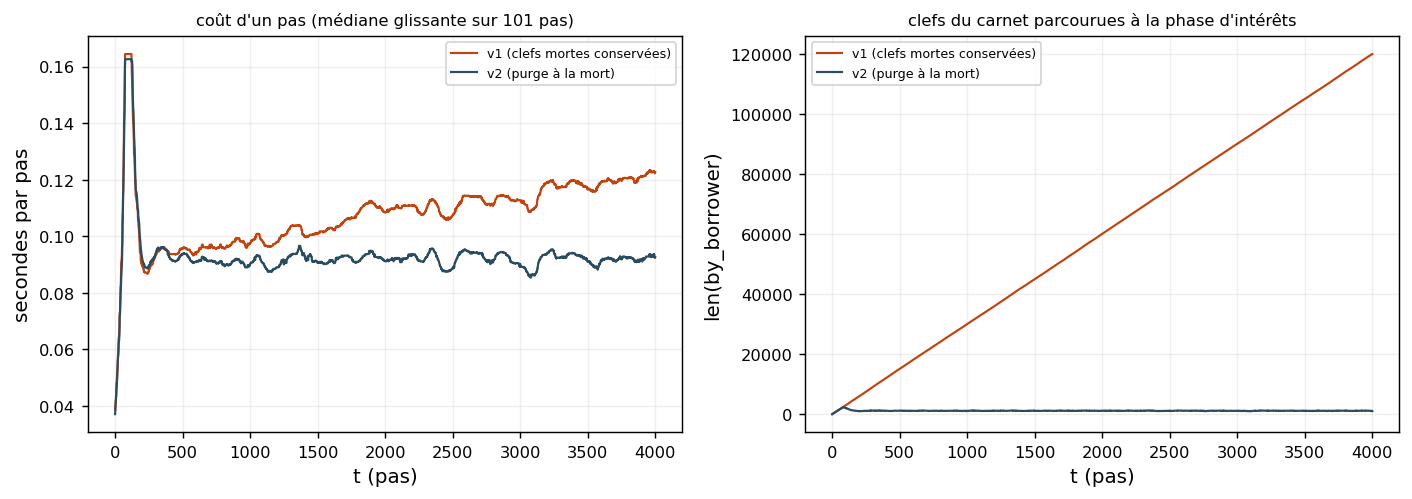
\includegraphics[width=\linewidth]{figures/cost_profile.png}
\caption{Coût par pas et taille du carnet, 4000 pas, graine 0, régime de
référence. Les deux moteurs tournent dans deux processus séparés, en
parallèle, chacun sur son cœur. Source :
\code{results/analysis/cost\_profile.csv}.}
\label{fig:cout}
\end{figure}

\fait{} Sur 4000 pas et à population constante, le carnet de v1 porte
\costVoneKeys{} clefs pour \costVonePop{} entités vivantes :
\textbf{\costEmptyShare\,\% sont vides}. Celui de v2 en porte
\costVtwoKeys{}, soit la population vivante à une unité près. Le coût par pas
de v1 est multiplié par \costVoneGrowth{} entre le début et la fin de
l'horizon (\costVoneEarly{} à \costVoneLate{}~ms) ; celui de v2 par
\costVtwoGrowth{}, c'est-à-dire qu'il ne croît pas. Le run entier passe de
\costVoneTotal{}~s à \costVtwoTotal{}~s, soit $-\costSaving\,\%$.

\incertitude{} Le coût par pas de v2 \emph{décroît} sur le même horizon. Ce n'est pas un effet de la purge : c'est le carnet \emph{actif} qui
se contracte après le transitoire initial, et v1 le subit aussi --- chez lui,
il est masqué par la croissance des clefs mortes. Le fait à retenir est que la
taille du carnet mort ne pilote plus rien.

\section{La borne de transfert supprimée}
\label{sec:plafond}

Le paramètre \code{transfer\_cap} n'avait que deux valeurs : \code{optimum},
l'énoncé littéral de l'institution, et \code{equalization}, un plafond du
transfert à $(K_\ell - K_b)/2$. \code{equalization} est retiré de v2 :
le tuple de validation, le champ de \code{Config}, la branche de plafonnement,
le compteur \code{mkt\_capped} et sa colonne, l'option de ligne de commande, et
le champ exposé par l'interface.

\fait{} \textbf{C'est du code mort, et c'est prouvé} : \code{mkt\_capped}
cumulé vaut \emph{exactement} 0 sur les runs v1 du dépôt. La suppression ne
peut donc changer aucun nombre publié, et la parité doit être reconduite telle
quelle. C'est précisément ce qui la distingue du chantier du sens
(§\ref{sec:concept-sens}), qui change réellement le comportement, et c'est
pourquoi elle est faite dans le premier lot, avant tout changement mesurable :
la parité qui suit porte alors sur un moteur déjà simplifié.

\paragraph{Le pilote de plafond de v1 reste publié, et il faut noter la
boucle.} Le rapport de conception de v1 documente \emph{pourquoi} le plafond
est sans objet : les entités dopées deviennent en quelques dizaines de pas le
côté riche de presque toutes leurs paires, l'optimum voudrait alors leur
envoyer du capital, et l'ancienne règle de sens l'interdisait. \inference{}
Ce raisonnement s'appuie donc sur la règle que v2 supprime. Il reste valable
comme justification historique, mais il ne peut plus servir d'argument sous le
sens libre : sous le sens libre, ces paires \emph{traitent}, en sens inverse.
La question « le plafond redevient-il pertinent ? » est donc rouverte en droit.
\incertitude{} Elle n'est pas tranchée ici, et le plafond n'est pas
réintroduit : il faudrait pour cela un motif institutionnel, pas seulement la
possibilité technique.

\section{L'ordre des phases, en option}
\label{sec:ordre-conception}

Le champ \code{phase\_order} vaut \code{"v1"} par défaut --- production,
service des intérêts, dépréciation --- ou \code{"deprec\_first"}, qui inverse
les deux dernières. La valeur par défaut préserve la parité sans détour ;
l'autre ne la préserve pas, et c'est le but.

L'implémentation extrait les deux phases en fonctions
(\code{\_service\_interest}, \code{\_depreciate}) appelées dans l'ordre voulu.
\fait{} L'extraction ne change aucun calcul : la parité bit à bit est
reconduite après.

\paragraph{Une prédiction que le moteur calcule lui-même.} Sous
\code{deprec\_first}, le capital disponible au moment de payer est réduit d'un
facteur $1-\delta$ : bascule en défaut de liquidité toute débitrice dont le
capital $K$ vérifie $(1-\delta)K < \mathrm{d\hat u} \le K$. C'est un ensemble
que le moteur peut compter \emph{dans le bras de référence lui-même} --- c'est
la colonne \code{defaults\_window}. Aucune division n'est employée :
$\mathrm{d\hat u} \le K/(1-\delta)$ est écrit
$\mathrm{d\hat u}\,(1-\delta) \le K$. La prédiction est donc écrite \emph{avant}
que le bras traité n'existe, ce qui est le seul moment où une prédiction a une
valeur.

\section{L'instrumentation devenue native}
\label{sec:instrumentation}

\subsection{La tension}
\label{sec:tension-native}

v1 satisfaisait la demande de tension \emph{a posteriori}, par un dérivé des
séries, parce que son moteur était gelé. Il devait reconstituer l'effectif
producteur par $n_{\text{vivantes}} + \text{morts}$, ce qui est exact tant
qu'une seule technologie vit et approché sinon ; une colonne \code{basis}
documentait laquelle des trois reconstructions avait servi.

v2 enregistre, par technologie et par pas, \code{n\_prod} et \code{K\_prod} ---
l'effectif et le capital \emph{à l'instant de produire}, après le choc
multiplicatif et avant que la production ne soit ajoutée au capital. La colonne
\code{basis} disparaît, faute d'ambiguïté à documenter.

\fait{} Deux gains de justesse, et non seulement de commodité. Le rapport de
Jensen $K_{\text{eq}}/\overline{K}$ devient exact, ses deux termes étant pris au
même instant du pas, là où v1 mélangeait la production et le capital de fin de
pas. Et le $\delta$ employé est celui du pas courant : un dérivé \emph{a
posteriori} lit un $\delta$ de fichier de configuration et ne verrait pas une
intervention sur $\delta$.

Le calcul vit dans \code{m4\_3live\_v2/tension.py}, module du \emph{moteur} et
non des scripts. Ce n'est pas un rangement : \code{scripts} est un nom de
premier niveau générique, et les deux lignées en ont un ; un import par nom
résoudrait vers l'une ou l'autre selon l'ordre de \code{sys.path}. Mettre le
calcul dans le paquet supprime la collision par construction. Le module de
tracé, lui, est chargé par chemin de fichier.

\subsection{L'amplitude exacte}
\label{sec:amplitude}

L'\textbf{amplitude} $m$ d'une intervention est le facteur par lequel elle
multiplie la production des entités qu'elle touche, au pas où elle agit pour la
première fois :
\begin{equation}
m \;=\;
\frac{\sum_{i \in \text{traitées}} A'_i K_i^{\gamma'_i}}
     {\sum_{i \in \text{traitées}} A_i K_i^{\gamma_i}},
\label{eq:amplitude}
\end{equation}
les deux sommes portant sur le \emph{même} capital $K_i$, celui de l'instant de
la production. v1 la reconstruisait depuis les agrégats ; v2 pose une sonde
$\{i \to (A_i, \gamma_i)\text{ d'avant}\}$ au moment de l'intervention et la
consomme dans la phase de production du même pas.

\paragraph{Une correction que la mesure a imposée.} \fait{} La sonde couvre
aussi les entités \emph{nées} au pas de l'intervention lorsque la technologie
de naissance a changé. Sans elles, la part de production traitée d'une portée
\code{all} vaut $0{,}9914$ au lieu de $1$ --- mesuré avant correction. La raison
est que ces entités portent déjà la nouvelle technologie mais n'auraient pas
existé avec l'ancienne : les omettre du contrefactuel revient à leur attribuer
la nouvelle production dans les deux branches.

\paragraph{Une identité, et pas une confirmation.} Le rapport
$E = (\Pi/\Pi_{\text{cf}} - 1)/((m-1)p)$, où $p$ est la part de production
\emph{ex ante} de la cohorte traitée, vaut 1 \textbf{par algèbre} : c'est une
réécriture des définitions de $m$ et de $p$. Son écart à 1 ne mesure que la
propreté de l'aller-retour flottant. C'est écrit dans la docstring de
\code{\_close\_amplitude} et redit dans le rapport de résultats, parce que
présenter une identité comme une confirmation empirique est exactement l'erreur
que v1 s'était signalée à elle-même.

\subsection{La prédiction naïve du levier \texorpdfstring{$\gamma$}{gamma}}

Pour tout levier sur $\gamma$, l'amplitude mesurée est enregistrée à côté de
deux prédictions : celle qu'on ferait en supposant $K = 1$ (où
$K^{\Delta\gamma} = 1$, donc « le levier ne fait rien »), et celle qu'on ferait
au capital équivalent, $K_{\text{eq}}^{\Delta\gamma}$.

\fait{} Sur un état de référence à $t = 200$, un levier $\gamma : 0{,}5 \to
0{,}6$ donne une amplitude mesurée de $1{,}960149$, contre $1{,}000000$ pour la
prédiction naïve et $1{,}952475$ pour la prédiction au capital équivalent
(écart $-0{,}39$\,\%). C'est le contenu informatif de la mesure : un levier sur
$\gamma$ n'est pas un cadran de puissance, et l'échelle de capital du système
suffit à le prédire à mieux que un demi pour cent.

\section{Les trois sémantiques de parité, et leur état}
\label{sec:parite}

C'est le point le plus facile à saboter par inattention, et les trois
sémantiques ne se confondent pas.

\begin{description}
\item[Parité obligatoire et bit-exacte (lot A).] Supprimer \code{equalization}
  retire du code qui n'a jamais été exécuté ; purger les clefs mortes supprime
  un \emph{no-op}. Toute déviation serait un bug de la suppression.
  \fait{} \textbf{Résultat : \parityLotASteps{} pas $\times$ 26 colonnes contre
  \code{m4\_3\_\_d1\_\_baseline\_\_seed0}, écart maximal \parityLotANul{}.}
  \parityLotACalls{} appels au noyau, tous sur le chemin identité --- exactement
  le nombre publié par v1. \parityLotASeconds{}~s, contre 1077~s pour v1 sur le
  même test (\code{results/analysis/parity\_lotA\_full.log}).
\item[Parité à retester, pas à supposer (lot B).] En régime homogène l'optimum
  est le partage égal, donc $\delta = (K_b - K_a)/2 \ge 0$ : le sens libre
  coïncide avec l'ancienne règle. Mais l'ordre du couple change l'ordre de
  sommation et d'insertion dans le carnet, et c'est le genre de détail qui
  décale un flottant.
  \fait{} \textbf{Résultat : parité reconduite, écart maximal
  \parityLotBCENul{}}, sur le moteur v2 complet avec le sens libre par défaut
  (\parityLotBCESeconds{}~s,
  \code{results/analysis/parity\_lotBCE\_full.log}).
\item[Parité conditionnelle (lot E).] Le défaut \code{phase\_order = "v1"} doit
  la préserver --- il la préserve, c'est la mesure ci-dessus. La branche
  \code{"deprec\_first"} ne la préserve pas, par construction.
\end{description}

\subsection{La seule différence, expliquée ligne à ligne}

\fait{} Le moteur v2 fait \parityLotBCECalls{} appels au noyau là où le lot A en
faisait \parityLotACalls{}, soit \textbf{$+2999$}. Aucune tolérance n'a été employée
pour absorber cet écart, parce qu'il ne porte sur aucun nombre.

L'explication est complète. v1 écartait les paires de capitaux égaux
\emph{avant} d'appeler le noyau (\code{if K[lender] <= K[borrower]: continue}).
v2 sous le sens libre les lui soumet, parce qu'entre technologies différentes
une paire de capitaux égaux a un optimum non trivial. En régime homogène, ces
2999 paires --- des entités à capital nul, mises à zéro par la dépréciation ---
reçoivent $\delta^{*} = 0$, sont comptées \code{blocked\_tiny} et ne traitent
pas. Aucune opération flottante n'est ajoutée à la trajectoire, et aucune table
du noyau n'est compilée différemment : le chemin identité ne tient pas de
compteur d'usage.

\subsection{La garantie qui compte vraiment pour la campagne}

\inference{} La parité avec M4.3 ne dit rien du régime hétérogène, qui est
justement celui où le sens du prêt a un objet. La garantie nécessaire est
autre : sous \code{loan\_direction="richest\_lends"}, le moteur v2 doit
reproduire le moteur v1 \emph{y compris} quand deux technologies coexistent.
Sans quoi la campagne A/B ne compare pas deux règles, mais deux lignées de code.

\fait{} C'est vérifié : 300 pas $\times$ \textbf{34 colonnes}, intervention
$A \times 1{,}5$ sur 20\,\% de la population à $t = 100$, deux technologies
vivantes, 61\,166 paires refusées pour cause de sens --- \textbf{écart
maximal NUL} entre le moteur v1 et v2 sous \code{richest\_lends}. Contrôle
négatif dans le même test : sous le sens libre, la première divergence tombe au
pas de l'intervention lui-même, et 30\,768 prêts sont conclus dans le sens
interdit.

\section{Ce que la suite de tests couvre}

Assertions Python simples, convention du dépôt --- pas de \code{pytest}.

\begin{center}\footnotesize
\begin{tabular}{@{}lp{10.2cm}@{}}
\toprule
\textbf{fichier} & \textbf{ce qu'il établit} \\
\midrule
\code{test\_parity\_m4\_3.py} & parité bit à bit avec M4.3, 26 colonnes ;
500 pas par défaut, 8000 avec \code{--full} \\
\code{test\_v1\_equivalence.py} & v2 sous \code{richest\_lends} reproduit le
moteur v1 en régime hétérogène ; contrôle négatif sous le sens libre \\
\code{test\_loan\_direction.py} & symétrie bit à bit du taux ; une paire
construite à la main où l'optimum exige que la moins riche cède ; le carnet, la
valeur nette et le compteur contrefactuel \\
\code{test\_tension.py} & formes fermées de $\Kaut$ et $K_{\text{eq}}$ ;
Jensen $=1$ exactement à capitaux égaux ; \code{n\_prod} $=$ vivantes $+$ morts
sur 400 pas ; agrégat pondéré par la production \\
\code{test\_amplitude.py} & amplitude exacte sur quatre leviers, part traitée,
prédiction naïve, et recalcul indépendant depuis les productions enregistrées \\
\code{test\_scale\_covariance.py} & covariance d'échelle : population et prêts
identiques, extensives à $3\times10^{-14}$ près, à deux $\gamma$ \\
\code{test\_institution.py} & les trois régimes du noyau contre forme fermée et
Newton ; ordre 4 de la table \\
\code{test\_scopes.py} & sémantique des portées, y compris les combinaisons
refusées \\
\code{test\_replay.py} & rejeu d'une session en direct réelle, invariant de
pause, pas-à-pas, aller-retour de snapshot \\
\code{test\_resume\_divergence.py} & reprise d'un run M4.3 stocké, écart mesuré
et non supposé \\
\code{test\_surplus\_rate.py} & règle de taux alternative $r = p\Delta/q$ \\
\code{test\_web\_live.py} & l'interface \code{/live2} de bout en bout par HTTP,
et la non-régression des routes de \code{simulation\_lab} et de v1 \\
\bottomrule
\end{tabular}
\end{center}

\incertitude{} \code{test\_web\_live.py} n'ouvre pas de navigateur et ne
regarde pas les pixels. Il démarre le serveur, crée une session, la fait
tourner, lui soumet une intervention, relit l'état par la route que le
navigateur emploie, et vérifie que chaque clef et chaque colonne que le
JavaScript consomme est présente. Le rendu graphique lui-même n'est pas testé.

\paragraph{Un défaut trouvé par ce test, et pas par la lecture.} \fait{} Le
préfixe des routes \code{POST} du routeur v2 était resté
\code{["api", "live", "sessions"]} après le renommage vers \code{/live2}, ce
qui rendait \emph{toutes} les actions de session --- jouer, mettre en pause,
intervenir, écrire --- inaccessibles. Les routes \code{GET} fonctionnaient, si
bien qu'une vérification par lecture de page n'aurait rien vu.

\section{Les décisions laissées ouvertes, et comment elles ont été tranchées}
\label{sec:decisions}

\begin{center}\footnotesize
\begin{tabular}{@{}p{3.5cm}p{4.2cm}p{6.0cm}@{}}
\toprule
\textbf{question} & \textbf{décision} & \textbf{ce qui la justifie} \\
\midrule
Nom du paquet forké &
\code{m4\_3live\_v2} &
Aucun conflit ; permet d'importer les deux moteurs dans un même processus. \\
\addlinespace
Le taux quand la créancière est la plus fragile &
\textbf{Règle inchangée} &
La formule est symétrique bit à bit : elle ne contient aucun rôle
(§\ref{sec:taux}). L'alternative « rendement marginal commun d'après
l'échange » est documentée et écartée. \\
\addlinespace
Nombre de graines de verdict &
\textbf{12} &
Coût \emph{mesuré} et non extrapolé : une cellule pilote de 2000 pas coûte
144,5~s sous le sens libre et 140,8~s sous la règle v1. La campagne
entière tient en une heure sur 7 processus. Seuil de Student à 11 degrés de
liberté : $2{,}201$ à 5\,\%, contre $2{,}776$ à 4 degrés. \\
\addlinespace
Rééchelonner \code{MIN\_LOAN} et \code{ZERO\_TOL} &
\textbf{Non} &
Cela rendrait la covariance d'échelle exacte, mais casserait la comparabilité
directe avec toutes les campagnes antérieures. Le gain ne se voit qu'au
quatorzième chiffre : l'écart résiduel mesuré est $3{,}1\times10^{-14}$
(\code{tests/test\_scale\_covariance.py}). \\
\addlinespace
La covariance de pas de temps devient-elle un test de non-régression ? &
\textbf{Non --- mais la covariance d'échelle, oui} &
Le résidu du recalage temporel est de 6 à 17\,\%, et sa source est la
phase de marché, qui ne se compose pas : un seuil y serait arbitraire. La
covariance d'échelle, elle, est exacte à $3\times10^{-14}$ : elle fait un test
légitime, et c'est \code{test\_scale\_covariance.py}. \\
\bottomrule
\end{tabular}
\end{center}

\section{Un trou assumé : les annotations de conception de v1}

La feuille de route de v2 réserve une section aux annotations que
l'utilisateur a portées sur le rapport de conception de v1. \fait{} Ce fichier
ne porte \emph{aucune} annotation sur le disque : zéro objet
\code{/Subtype/Text}, vérifié par \code{pdftk dump\_data\_annots} et par
\code{mutool show}. L'horodatage du fichier est celui de sa compilation,
antérieur à la première note du rapport final.

\inference{} Les annotations n'ont vraisemblablement pas été enregistrées
depuis la visionneuse. Rien n'a été inventé pour combler ce trou. Si une copie
annotée est fournie, elle sera intégrée ; en attendant, le présent document est
\textbf{incomplet d'un jeu de retours}, et c'est dit ici plutôt que passé sous
silence.

\section{Périmètre : ce qui a été retiré, et à la demande de qui}

\begin{itemize}
\item \textbf{Aucun traitement du cas partiel.} La portée \code{fraction}
  reste dans le moteur --- elle est testée, elle fonctionne --- mais aucune
  campagne de v2 ne l'emploie. Sortent avec elle : les bras \code{null}
  appariés, l'inversion de la part traitée \emph{ex post} en part \emph{ex
  ante}, et la question du long horizon posée en portée partielle. v2 mesure en
  portée globale, où l'intensité de traitement vaut 1 par construction.
\item \textbf{Une seule borne de transfert.} §\ref{sec:plafond}.
\end{itemize}

Les résultats de v1 obtenus en portée partielle restent acquis et publiés ; ils
ne sont simplement pas prolongés.

\section{Un écart au séquencement demandé, et sa portée}

\incertitude{} Le prompt demande que les lots qui changent le modèle soient
\emph{séparés dans l'historique git}. L'historique de v2 comporte le fork, puis
le lot A seul, puis les lots B, C et E groupés dans un même commit --- ils ont
été écrits dans une même passe d'édition sur un seul fichier.

Ce qui est en jeu est l'attribution des verdicts, et elle n'en dépend pas :
elle est assurée par des \textbf{drapeaux d'exécution}. La campagne du sens du
prêt oppose \code{loan\_direction="free"} à \code{"richest\_lends"} dans le
\emph{même binaire}, sur les \emph{mêmes} snapshots et les \emph{mêmes}
graines ; celle de l'ordre des phases oppose de même
\code{phase\_order="v1"} à \code{"deprec\_first"}. C'est plus fort qu'une
séparation d'historique, qui ne garantirait qu'une chose : que les deux
versions ont existé séparément. Le lot C, lui, est de l'instrumentation et ne
change aucune trajectoire --- la parité bit à bit le vérifie.

\section{Reproduire}
\label{sec:reproduire-conception}

Toutes les commandes partent de \code{/home/anatole/jupyter} avec
\code{PY=/home/anatole/jupyter/.venv/bin/python3}.

\begin{center}\footnotesize
\begin{tabular}{@{}p{9.4cm}p{4.2cm}@{}}
\toprule
\textbf{commande} & \textbf{coût mesuré} \\
\midrule
\code{\$PY m4\_3live\_v2\_credit\_soc/tests/test\_parity\_m4\_3.py --full} &
741~s \\
\code{\$PY m4\_3live\_v2\_credit\_soc/tests/test\_v1\_equivalence.py} &
59~s \\
\code{\$PY m4\_3live\_v2\_credit\_soc/tests/test\_loan\_direction.py} &
$<$~1~s \\
\code{\$PY m4\_3live\_v2\_credit\_soc/tests/test\_tension.py} & 25~s \\
\code{\$PY m4\_3live\_v2\_credit\_soc/tests/test\_amplitude.py} & 60~s \\
\code{\$PY m4\_3live\_v2\_credit\_soc/tests/test\_scale\_covariance.py} &
200~s \\
\code{\$PY m4\_3live\_v2\_credit\_soc/tests/test\_web\_live.py} & 30~s \\
\code{\$PY m4\_3live\_v2\_credit\_soc/scripts/cost\_profile.py --steps 4000} &
447~s (2 processus) \\
\bottomrule
\end{tabular}
\end{center}

\noindent Le protocole des campagnes et le coût de chacune sont donnés dans le
rapport de résultats, section « Reproduire ».

\appendix
\section{Annexe de traçabilité}
\label{sec:tracabilite-conception}

Toute simulation citée dans ce document est identifiable par son
\code{run\_id} dans \code{simulation\_lab}. Les renvois sont des
\emph{sections} et jamais des numéros de figure. Le tableau est engendré par
\code{scripts/make\_traceability.py}, qui refuse de produire une annexe dont
une ligne serait sans rôle.

{\scriptsize
\setlength{\tabcolsep}{4pt}
\begin{longtable}{@{}>{\raggedright\arraybackslash}p{5.3cm}>{\raggedright\arraybackslash}p{1.9cm}>{\raggedright\arraybackslash}p{3.2cm}>{\raggedright\arraybackslash}p{4.9cm}@{}}
\toprule
\textbf{run\_id (simulation\_lab)} & \textbf{groupe} & \textbf{apparaît dans} & \textbf{rôle / interventions} \\
\midrule
\endfirsthead
\toprule
\textbf{run\_id (simulation\_lab)} & \textbf{groupe} & \textbf{apparaît dans} & \textbf{rôle / interventions} \\
\midrule
\endhead
\code{m4\_3live\_v2\_\_\allowbreak{}arm\_\_\allowbreak{}free\_\_\allowbreak{}all\_A150\_\_\allowbreak{}seed0} & lot D & campagne A/B & hausse globale $A\textbackslash{}times1{,}5$ : reste homogène, donc insensible à la règle de sens \\ \textit{t=2001 A$\rightarrow$1.5 (all)} \\
\code{m4\_3live\_v2\_\_\allowbreak{}arm\_\_\allowbreak{}free\_\_\allowbreak{}all\_A150\_\_\allowbreak{}seed1} & lot D & campagne A/B & hausse globale $A\textbackslash{}times1{,}5$ : reste homogène, donc insensible à la règle de sens \\ \textit{t=2001 A$\rightarrow$1.5 (all)} \\
\code{m4\_3live\_v2\_\_\allowbreak{}arm\_\_\allowbreak{}free\_\_\allowbreak{}all\_A150\_\_\allowbreak{}seed10} & lot D & campagne A/B & hausse globale $A\textbackslash{}times1{,}5$ : reste homogène, donc insensible à la règle de sens \\ \textit{t=2001 A$\rightarrow$1.5 (all)} \\
\code{m4\_3live\_v2\_\_\allowbreak{}arm\_\_\allowbreak{}free\_\_\allowbreak{}all\_A150\_\_\allowbreak{}seed11} & lot D & campagne A/B & hausse globale $A\textbackslash{}times1{,}5$ : reste homogène, donc insensible à la règle de sens \\ \textit{t=2001 A$\rightarrow$1.5 (all)} \\
\code{m4\_3live\_v2\_\_\allowbreak{}arm\_\_\allowbreak{}free\_\_\allowbreak{}all\_A150\_\_\allowbreak{}seed2} & lot D & campagne A/B & hausse globale $A\textbackslash{}times1{,}5$ : reste homogène, donc insensible à la règle de sens \\ \textit{t=2001 A$\rightarrow$1.5 (all)} \\
\code{m4\_3live\_v2\_\_\allowbreak{}arm\_\_\allowbreak{}free\_\_\allowbreak{}all\_A150\_\_\allowbreak{}seed3} & lot D & campagne A/B & hausse globale $A\textbackslash{}times1{,}5$ : reste homogène, donc insensible à la règle de sens \\ \textit{t=2001 A$\rightarrow$1.5 (all)} \\
\code{m4\_3live\_v2\_\_\allowbreak{}arm\_\_\allowbreak{}free\_\_\allowbreak{}all\_A150\_\_\allowbreak{}seed4} & lot D & campagne A/B & hausse globale $A\textbackslash{}times1{,}5$ : reste homogène, donc insensible à la règle de sens \\ \textit{t=2001 A$\rightarrow$1.5 (all)} \\
\code{m4\_3live\_v2\_\_\allowbreak{}arm\_\_\allowbreak{}free\_\_\allowbreak{}all\_A150\_\_\allowbreak{}seed5} & lot D & campagne A/B & hausse globale $A\textbackslash{}times1{,}5$ : reste homogène, donc insensible à la règle de sens \\ \textit{t=2001 A$\rightarrow$1.5 (all)} \\
\code{m4\_3live\_v2\_\_\allowbreak{}arm\_\_\allowbreak{}free\_\_\allowbreak{}all\_A150\_\_\allowbreak{}seed6} & lot D & campagne A/B & hausse globale $A\textbackslash{}times1{,}5$ : reste homogène, donc insensible à la règle de sens \\ \textit{t=2001 A$\rightarrow$1.5 (all)} \\
\code{m4\_3live\_v2\_\_\allowbreak{}arm\_\_\allowbreak{}free\_\_\allowbreak{}all\_A150\_\_\allowbreak{}seed7} & lot D & campagne A/B & hausse globale $A\textbackslash{}times1{,}5$ : reste homogène, donc insensible à la règle de sens \\ \textit{t=2001 A$\rightarrow$1.5 (all)} \\
\code{m4\_3live\_v2\_\_\allowbreak{}arm\_\_\allowbreak{}free\_\_\allowbreak{}all\_A150\_\_\allowbreak{}seed8} & lot D & campagne A/B & hausse globale $A\textbackslash{}times1{,}5$ : reste homogène, donc insensible à la règle de sens \\ \textit{t=2001 A$\rightarrow$1.5 (all)} \\
\code{m4\_3live\_v2\_\_\allowbreak{}arm\_\_\allowbreak{}free\_\_\allowbreak{}all\_A150\_\_\allowbreak{}seed9} & lot D & campagne A/B & hausse globale $A\textbackslash{}times1{,}5$ : reste homogène, donc insensible à la règle de sens \\ \textit{t=2001 A$\rightarrow$1.5 (all)} \\
\code{m4\_3live\_v2\_\_\allowbreak{}arm\_\_\allowbreak{}free\_\_\allowbreak{}control\_\_\allowbreak{}seed0} & lot D & campagne A/B ; contrôle de stationnarité & référence inerte sous sens libre \\
\code{m4\_3live\_v2\_\_\allowbreak{}arm\_\_\allowbreak{}free\_\_\allowbreak{}control\_\_\allowbreak{}seed1} & lot D & campagne A/B ; contrôle de stationnarité & référence inerte sous sens libre \\
\code{m4\_3live\_v2\_\_\allowbreak{}arm\_\_\allowbreak{}free\_\_\allowbreak{}control\_\_\allowbreak{}seed10} & lot D & campagne A/B ; contrôle de stationnarité & référence inerte sous sens libre \\
\code{m4\_3live\_v2\_\_\allowbreak{}arm\_\_\allowbreak{}free\_\_\allowbreak{}control\_\_\allowbreak{}seed11} & lot D & campagne A/B ; contrôle de stationnarité & référence inerte sous sens libre \\
\code{m4\_3live\_v2\_\_\allowbreak{}arm\_\_\allowbreak{}free\_\_\allowbreak{}control\_\_\allowbreak{}seed2} & lot D & campagne A/B ; contrôle de stationnarité & référence inerte sous sens libre \\
\code{m4\_3live\_v2\_\_\allowbreak{}arm\_\_\allowbreak{}free\_\_\allowbreak{}control\_\_\allowbreak{}seed3} & lot D & campagne A/B ; contrôle de stationnarité & référence inerte sous sens libre \\
\code{m4\_3live\_v2\_\_\allowbreak{}arm\_\_\allowbreak{}free\_\_\allowbreak{}control\_\_\allowbreak{}seed4} & lot D & campagne A/B ; contrôle de stationnarité & référence inerte sous sens libre \\
\code{m4\_3live\_v2\_\_\allowbreak{}arm\_\_\allowbreak{}free\_\_\allowbreak{}control\_\_\allowbreak{}seed5} & lot D & campagne A/B ; contrôle de stationnarité & référence inerte sous sens libre \\
\code{m4\_3live\_v2\_\_\allowbreak{}arm\_\_\allowbreak{}free\_\_\allowbreak{}control\_\_\allowbreak{}seed6} & lot D & campagne A/B ; contrôle de stationnarité & référence inerte sous sens libre \\
\code{m4\_3live\_v2\_\_\allowbreak{}arm\_\_\allowbreak{}free\_\_\allowbreak{}control\_\_\allowbreak{}seed7} & lot D & campagne A/B ; contrôle de stationnarité & référence inerte sous sens libre \\
\code{m4\_3live\_v2\_\_\allowbreak{}arm\_\_\allowbreak{}free\_\_\allowbreak{}control\_\_\allowbreak{}seed8} & lot D & campagne A/B ; contrôle de stationnarité & référence inerte sous sens libre \\
\code{m4\_3live\_v2\_\_\allowbreak{}arm\_\_\allowbreak{}free\_\_\allowbreak{}control\_\_\allowbreak{}seed9} & lot D & campagne A/B ; contrôle de stationnarité & référence inerte sous sens libre \\
\code{m4\_3live\_v2\_\_\allowbreak{}arm\_\_\allowbreak{}free\_\_\allowbreak{}new\_A075\_\_\allowbreak{}seed0} & lot D & campagne A/B & vintage $A\textbackslash{}times0{,}75$, sens libre \\ \textit{t=2001 A$\rightarrow$0.75 (new)} \\
\code{m4\_3live\_v2\_\_\allowbreak{}arm\_\_\allowbreak{}free\_\_\allowbreak{}new\_A075\_\_\allowbreak{}seed1} & lot D & campagne A/B & vintage $A\textbackslash{}times0{,}75$, sens libre \\ \textit{t=2001 A$\rightarrow$0.75 (new)} \\
\code{m4\_3live\_v2\_\_\allowbreak{}arm\_\_\allowbreak{}free\_\_\allowbreak{}new\_A075\_\_\allowbreak{}seed10} & lot D & campagne A/B & vintage $A\textbackslash{}times0{,}75$, sens libre \\ \textit{t=2001 A$\rightarrow$0.75 (new)} \\
\code{m4\_3live\_v2\_\_\allowbreak{}arm\_\_\allowbreak{}free\_\_\allowbreak{}new\_A075\_\_\allowbreak{}seed11} & lot D & campagne A/B & vintage $A\textbackslash{}times0{,}75$, sens libre \\ \textit{t=2001 A$\rightarrow$0.75 (new)} \\
\code{m4\_3live\_v2\_\_\allowbreak{}arm\_\_\allowbreak{}free\_\_\allowbreak{}new\_A075\_\_\allowbreak{}seed2} & lot D & campagne A/B & vintage $A\textbackslash{}times0{,}75$, sens libre \\ \textit{t=2001 A$\rightarrow$0.75 (new)} \\
\code{m4\_3live\_v2\_\_\allowbreak{}arm\_\_\allowbreak{}free\_\_\allowbreak{}new\_A075\_\_\allowbreak{}seed3} & lot D & campagne A/B & vintage $A\textbackslash{}times0{,}75$, sens libre \\ \textit{t=2001 A$\rightarrow$0.75 (new)} \\
\code{m4\_3live\_v2\_\_\allowbreak{}arm\_\_\allowbreak{}free\_\_\allowbreak{}new\_A075\_\_\allowbreak{}seed4} & lot D & campagne A/B & vintage $A\textbackslash{}times0{,}75$, sens libre \\ \textit{t=2001 A$\rightarrow$0.75 (new)} \\
\code{m4\_3live\_v2\_\_\allowbreak{}arm\_\_\allowbreak{}free\_\_\allowbreak{}new\_A075\_\_\allowbreak{}seed5} & lot D & campagne A/B & vintage $A\textbackslash{}times0{,}75$, sens libre \\ \textit{t=2001 A$\rightarrow$0.75 (new)} \\
\code{m4\_3live\_v2\_\_\allowbreak{}arm\_\_\allowbreak{}free\_\_\allowbreak{}new\_A075\_\_\allowbreak{}seed6} & lot D & campagne A/B & vintage $A\textbackslash{}times0{,}75$, sens libre \\ \textit{t=2001 A$\rightarrow$0.75 (new)} \\
\code{m4\_3live\_v2\_\_\allowbreak{}arm\_\_\allowbreak{}free\_\_\allowbreak{}new\_A075\_\_\allowbreak{}seed7} & lot D & campagne A/B & vintage $A\textbackslash{}times0{,}75$, sens libre \\ \textit{t=2001 A$\rightarrow$0.75 (new)} \\
\code{m4\_3live\_v2\_\_\allowbreak{}arm\_\_\allowbreak{}free\_\_\allowbreak{}new\_A075\_\_\allowbreak{}seed8} & lot D & campagne A/B & vintage $A\textbackslash{}times0{,}75$, sens libre \\ \textit{t=2001 A$\rightarrow$0.75 (new)} \\
\code{m4\_3live\_v2\_\_\allowbreak{}arm\_\_\allowbreak{}free\_\_\allowbreak{}new\_A075\_\_\allowbreak{}seed9} & lot D & campagne A/B & vintage $A\textbackslash{}times0{,}75$, sens libre \\ \textit{t=2001 A$\rightarrow$0.75 (new)} \\
\code{m4\_3live\_v2\_\_\allowbreak{}arm\_\_\allowbreak{}free\_\_\allowbreak{}new\_A150\_\_\allowbreak{}seed0} & lot D & campagne A/B ; régime nouveau & vintage $A\textbackslash{}times1{,}5$, sens libre \\ \textit{t=2001 A$\rightarrow$1.5 (new)} \\
\code{m4\_3live\_v2\_\_\allowbreak{}arm\_\_\allowbreak{}free\_\_\allowbreak{}new\_A150\_\_\allowbreak{}seed1} & lot D & campagne A/B ; régime nouveau & vintage $A\textbackslash{}times1{,}5$, sens libre \\ \textit{t=2001 A$\rightarrow$1.5 (new)} \\
\code{m4\_3live\_v2\_\_\allowbreak{}arm\_\_\allowbreak{}free\_\_\allowbreak{}new\_A150\_\_\allowbreak{}seed10} & lot D & campagne A/B ; régime nouveau & vintage $A\textbackslash{}times1{,}5$, sens libre \\ \textit{t=2001 A$\rightarrow$1.5 (new)} \\
\code{m4\_3live\_v2\_\_\allowbreak{}arm\_\_\allowbreak{}free\_\_\allowbreak{}new\_A150\_\_\allowbreak{}seed11} & lot D & campagne A/B ; régime nouveau & vintage $A\textbackslash{}times1{,}5$, sens libre \\ \textit{t=2001 A$\rightarrow$1.5 (new)} \\
\code{m4\_3live\_v2\_\_\allowbreak{}arm\_\_\allowbreak{}free\_\_\allowbreak{}new\_A150\_\_\allowbreak{}seed2} & lot D & campagne A/B ; régime nouveau & vintage $A\textbackslash{}times1{,}5$, sens libre \\ \textit{t=2001 A$\rightarrow$1.5 (new)} \\
\code{m4\_3live\_v2\_\_\allowbreak{}arm\_\_\allowbreak{}free\_\_\allowbreak{}new\_A150\_\_\allowbreak{}seed3} & lot D & campagne A/B ; régime nouveau & vintage $A\textbackslash{}times1{,}5$, sens libre \\ \textit{t=2001 A$\rightarrow$1.5 (new)} \\
\code{m4\_3live\_v2\_\_\allowbreak{}arm\_\_\allowbreak{}free\_\_\allowbreak{}new\_A150\_\_\allowbreak{}seed4} & lot D & campagne A/B ; régime nouveau & vintage $A\textbackslash{}times1{,}5$, sens libre \\ \textit{t=2001 A$\rightarrow$1.5 (new)} \\
\code{m4\_3live\_v2\_\_\allowbreak{}arm\_\_\allowbreak{}free\_\_\allowbreak{}new\_A150\_\_\allowbreak{}seed5} & lot D & campagne A/B ; régime nouveau & vintage $A\textbackslash{}times1{,}5$, sens libre \\ \textit{t=2001 A$\rightarrow$1.5 (new)} \\
\code{m4\_3live\_v2\_\_\allowbreak{}arm\_\_\allowbreak{}free\_\_\allowbreak{}new\_A150\_\_\allowbreak{}seed6} & lot D & campagne A/B ; régime nouveau & vintage $A\textbackslash{}times1{,}5$, sens libre \\ \textit{t=2001 A$\rightarrow$1.5 (new)} \\
\code{m4\_3live\_v2\_\_\allowbreak{}arm\_\_\allowbreak{}free\_\_\allowbreak{}new\_A150\_\_\allowbreak{}seed7} & lot D & campagne A/B ; régime nouveau & vintage $A\textbackslash{}times1{,}5$, sens libre \\ \textit{t=2001 A$\rightarrow$1.5 (new)} \\
\code{m4\_3live\_v2\_\_\allowbreak{}arm\_\_\allowbreak{}free\_\_\allowbreak{}new\_A150\_\_\allowbreak{}seed8} & lot D & campagne A/B ; régime nouveau & vintage $A\textbackslash{}times1{,}5$, sens libre \\ \textit{t=2001 A$\rightarrow$1.5 (new)} \\
\code{m4\_3live\_v2\_\_\allowbreak{}arm\_\_\allowbreak{}free\_\_\allowbreak{}new\_A150\_\_\allowbreak{}seed9} & lot D & campagne A/B ; régime nouveau & vintage $A\textbackslash{}times1{,}5$, sens libre \\ \textit{t=2001 A$\rightarrow$1.5 (new)} \\
\code{m4\_3live\_v2\_\_\allowbreak{}arm\_\_\allowbreak{}free\_\_\allowbreak{}new\_g060\_\_\allowbreak{}seed0} & lot D & campagne A/B & vintage $\textbackslash{}gamma : 0{,}5 \textbackslash{}to 0{,}6$, sens libre ; exerce le régime (c) du noyau \\ \textit{t=2001 gamma$\rightarrow$0.6 (new)} \\
\code{m4\_3live\_v2\_\_\allowbreak{}arm\_\_\allowbreak{}free\_\_\allowbreak{}new\_g060\_\_\allowbreak{}seed1} & lot D & campagne A/B & vintage $\textbackslash{}gamma : 0{,}5 \textbackslash{}to 0{,}6$, sens libre ; exerce le régime (c) du noyau \\ \textit{t=2001 gamma$\rightarrow$0.6 (new)} \\
\code{m4\_3live\_v2\_\_\allowbreak{}arm\_\_\allowbreak{}free\_\_\allowbreak{}new\_g060\_\_\allowbreak{}seed10} & lot D & campagne A/B & vintage $\textbackslash{}gamma : 0{,}5 \textbackslash{}to 0{,}6$, sens libre ; exerce le régime (c) du noyau \\ \textit{t=2001 gamma$\rightarrow$0.6 (new)} \\
\code{m4\_3live\_v2\_\_\allowbreak{}arm\_\_\allowbreak{}free\_\_\allowbreak{}new\_g060\_\_\allowbreak{}seed11} & lot D & campagne A/B & vintage $\textbackslash{}gamma : 0{,}5 \textbackslash{}to 0{,}6$, sens libre ; exerce le régime (c) du noyau \\ \textit{t=2001 gamma$\rightarrow$0.6 (new)} \\
\code{m4\_3live\_v2\_\_\allowbreak{}arm\_\_\allowbreak{}free\_\_\allowbreak{}new\_g060\_\_\allowbreak{}seed2} & lot D & campagne A/B & vintage $\textbackslash{}gamma : 0{,}5 \textbackslash{}to 0{,}6$, sens libre ; exerce le régime (c) du noyau \\ \textit{t=2001 gamma$\rightarrow$0.6 (new)} \\
\code{m4\_3live\_v2\_\_\allowbreak{}arm\_\_\allowbreak{}free\_\_\allowbreak{}new\_g060\_\_\allowbreak{}seed3} & lot D & campagne A/B & vintage $\textbackslash{}gamma : 0{,}5 \textbackslash{}to 0{,}6$, sens libre ; exerce le régime (c) du noyau \\ \textit{t=2001 gamma$\rightarrow$0.6 (new)} \\
\code{m4\_3live\_v2\_\_\allowbreak{}arm\_\_\allowbreak{}free\_\_\allowbreak{}new\_g060\_\_\allowbreak{}seed4} & lot D & campagne A/B & vintage $\textbackslash{}gamma : 0{,}5 \textbackslash{}to 0{,}6$, sens libre ; exerce le régime (c) du noyau \\ \textit{t=2001 gamma$\rightarrow$0.6 (new)} \\
\code{m4\_3live\_v2\_\_\allowbreak{}arm\_\_\allowbreak{}free\_\_\allowbreak{}new\_g060\_\_\allowbreak{}seed5} & lot D & campagne A/B & vintage $\textbackslash{}gamma : 0{,}5 \textbackslash{}to 0{,}6$, sens libre ; exerce le régime (c) du noyau \\ \textit{t=2001 gamma$\rightarrow$0.6 (new)} \\
\code{m4\_3live\_v2\_\_\allowbreak{}arm\_\_\allowbreak{}free\_\_\allowbreak{}new\_g060\_\_\allowbreak{}seed6} & lot D & campagne A/B & vintage $\textbackslash{}gamma : 0{,}5 \textbackslash{}to 0{,}6$, sens libre ; exerce le régime (c) du noyau \\ \textit{t=2001 gamma$\rightarrow$0.6 (new)} \\
\code{m4\_3live\_v2\_\_\allowbreak{}arm\_\_\allowbreak{}free\_\_\allowbreak{}new\_g060\_\_\allowbreak{}seed7} & lot D & campagne A/B & vintage $\textbackslash{}gamma : 0{,}5 \textbackslash{}to 0{,}6$, sens libre ; exerce le régime (c) du noyau \\ \textit{t=2001 gamma$\rightarrow$0.6 (new)} \\
\code{m4\_3live\_v2\_\_\allowbreak{}arm\_\_\allowbreak{}free\_\_\allowbreak{}new\_g060\_\_\allowbreak{}seed8} & lot D & campagne A/B & vintage $\textbackslash{}gamma : 0{,}5 \textbackslash{}to 0{,}6$, sens libre ; exerce le régime (c) du noyau \\ \textit{t=2001 gamma$\rightarrow$0.6 (new)} \\
\code{m4\_3live\_v2\_\_\allowbreak{}arm\_\_\allowbreak{}free\_\_\allowbreak{}new\_g060\_\_\allowbreak{}seed9} & lot D & campagne A/B & vintage $\textbackslash{}gamma : 0{,}5 \textbackslash{}to 0{,}6$, sens libre ; exerce le régime (c) du noyau \\ \textit{t=2001 gamma$\rightarrow$0.6 (new)} \\
\code{m4\_3live\_v2\_\_\allowbreak{}arm\_\_\allowbreak{}richest\_lends\_\_\allowbreak{}new\_A075\_\_\allowbreak{}seed0} & lot D & campagne A/B & même bras sous la règle v1 \\ \textit{t=2001 A$\rightarrow$0.75 (new)} \\
\code{m4\_3live\_v2\_\_\allowbreak{}arm\_\_\allowbreak{}richest\_lends\_\_\allowbreak{}new\_A075\_\_\allowbreak{}seed1} & lot D & campagne A/B & même bras sous la règle v1 \\ \textit{t=2001 A$\rightarrow$0.75 (new)} \\
\code{m4\_3live\_v2\_\_\allowbreak{}arm\_\_\allowbreak{}richest\_lends\_\_\allowbreak{}new\_A075\_\_\allowbreak{}seed10} & lot D & campagne A/B & même bras sous la règle v1 \\ \textit{t=2001 A$\rightarrow$0.75 (new)} \\
\code{m4\_3live\_v2\_\_\allowbreak{}arm\_\_\allowbreak{}richest\_lends\_\_\allowbreak{}new\_A075\_\_\allowbreak{}seed11} & lot D & campagne A/B & même bras sous la règle v1 \\ \textit{t=2001 A$\rightarrow$0.75 (new)} \\
\code{m4\_3live\_v2\_\_\allowbreak{}arm\_\_\allowbreak{}richest\_lends\_\_\allowbreak{}new\_A075\_\_\allowbreak{}seed2} & lot D & campagne A/B & même bras sous la règle v1 \\ \textit{t=2001 A$\rightarrow$0.75 (new)} \\
\code{m4\_3live\_v2\_\_\allowbreak{}arm\_\_\allowbreak{}richest\_lends\_\_\allowbreak{}new\_A075\_\_\allowbreak{}seed3} & lot D & campagne A/B & même bras sous la règle v1 \\ \textit{t=2001 A$\rightarrow$0.75 (new)} \\
\code{m4\_3live\_v2\_\_\allowbreak{}arm\_\_\allowbreak{}richest\_lends\_\_\allowbreak{}new\_A075\_\_\allowbreak{}seed4} & lot D & campagne A/B & même bras sous la règle v1 \\ \textit{t=2001 A$\rightarrow$0.75 (new)} \\
\code{m4\_3live\_v2\_\_\allowbreak{}arm\_\_\allowbreak{}richest\_lends\_\_\allowbreak{}new\_A075\_\_\allowbreak{}seed5} & lot D & campagne A/B & même bras sous la règle v1 \\ \textit{t=2001 A$\rightarrow$0.75 (new)} \\
\code{m4\_3live\_v2\_\_\allowbreak{}arm\_\_\allowbreak{}richest\_lends\_\_\allowbreak{}new\_A075\_\_\allowbreak{}seed6} & lot D & campagne A/B & même bras sous la règle v1 \\ \textit{t=2001 A$\rightarrow$0.75 (new)} \\
\code{m4\_3live\_v2\_\_\allowbreak{}arm\_\_\allowbreak{}richest\_lends\_\_\allowbreak{}new\_A075\_\_\allowbreak{}seed7} & lot D & campagne A/B & même bras sous la règle v1 \\ \textit{t=2001 A$\rightarrow$0.75 (new)} \\
\code{m4\_3live\_v2\_\_\allowbreak{}arm\_\_\allowbreak{}richest\_lends\_\_\allowbreak{}new\_A075\_\_\allowbreak{}seed8} & lot D & campagne A/B & même bras sous la règle v1 \\ \textit{t=2001 A$\rightarrow$0.75 (new)} \\
\code{m4\_3live\_v2\_\_\allowbreak{}arm\_\_\allowbreak{}richest\_lends\_\_\allowbreak{}new\_A075\_\_\allowbreak{}seed9} & lot D & campagne A/B & même bras sous la règle v1 \\ \textit{t=2001 A$\rightarrow$0.75 (new)} \\
\code{m4\_3live\_v2\_\_\allowbreak{}arm\_\_\allowbreak{}richest\_lends\_\_\allowbreak{}new\_A150\_\_\allowbreak{}seed0} & lot D & campagne A/B & même bras sous la règle v1 « la plus riche prête » \\ \textit{t=2001 A$\rightarrow$1.5 (new)} \\
\code{m4\_3live\_v2\_\_\allowbreak{}arm\_\_\allowbreak{}richest\_lends\_\_\allowbreak{}new\_A150\_\_\allowbreak{}seed1} & lot D & campagne A/B & même bras sous la règle v1 « la plus riche prête » \\ \textit{t=2001 A$\rightarrow$1.5 (new)} \\
\code{m4\_3live\_v2\_\_\allowbreak{}arm\_\_\allowbreak{}richest\_lends\_\_\allowbreak{}new\_A150\_\_\allowbreak{}seed10} & lot D & campagne A/B & même bras sous la règle v1 « la plus riche prête » \\ \textit{t=2001 A$\rightarrow$1.5 (new)} \\
\code{m4\_3live\_v2\_\_\allowbreak{}arm\_\_\allowbreak{}richest\_lends\_\_\allowbreak{}new\_A150\_\_\allowbreak{}seed11} & lot D & campagne A/B & même bras sous la règle v1 « la plus riche prête » \\ \textit{t=2001 A$\rightarrow$1.5 (new)} \\
\code{m4\_3live\_v2\_\_\allowbreak{}arm\_\_\allowbreak{}richest\_lends\_\_\allowbreak{}new\_A150\_\_\allowbreak{}seed2} & lot D & campagne A/B & même bras sous la règle v1 « la plus riche prête » \\ \textit{t=2001 A$\rightarrow$1.5 (new)} \\
\code{m4\_3live\_v2\_\_\allowbreak{}arm\_\_\allowbreak{}richest\_lends\_\_\allowbreak{}new\_A150\_\_\allowbreak{}seed3} & lot D & campagne A/B & même bras sous la règle v1 « la plus riche prête » \\ \textit{t=2001 A$\rightarrow$1.5 (new)} \\
\code{m4\_3live\_v2\_\_\allowbreak{}arm\_\_\allowbreak{}richest\_lends\_\_\allowbreak{}new\_A150\_\_\allowbreak{}seed4} & lot D & campagne A/B & même bras sous la règle v1 « la plus riche prête » \\ \textit{t=2001 A$\rightarrow$1.5 (new)} \\
\code{m4\_3live\_v2\_\_\allowbreak{}arm\_\_\allowbreak{}richest\_lends\_\_\allowbreak{}new\_A150\_\_\allowbreak{}seed5} & lot D & campagne A/B & même bras sous la règle v1 « la plus riche prête » \\ \textit{t=2001 A$\rightarrow$1.5 (new)} \\
\code{m4\_3live\_v2\_\_\allowbreak{}arm\_\_\allowbreak{}richest\_lends\_\_\allowbreak{}new\_A150\_\_\allowbreak{}seed6} & lot D & campagne A/B & même bras sous la règle v1 « la plus riche prête » \\ \textit{t=2001 A$\rightarrow$1.5 (new)} \\
\code{m4\_3live\_v2\_\_\allowbreak{}arm\_\_\allowbreak{}richest\_lends\_\_\allowbreak{}new\_A150\_\_\allowbreak{}seed7} & lot D & campagne A/B & même bras sous la règle v1 « la plus riche prête » \\ \textit{t=2001 A$\rightarrow$1.5 (new)} \\
\code{m4\_3live\_v2\_\_\allowbreak{}arm\_\_\allowbreak{}richest\_lends\_\_\allowbreak{}new\_A150\_\_\allowbreak{}seed8} & lot D & campagne A/B & même bras sous la règle v1 « la plus riche prête » \\ \textit{t=2001 A$\rightarrow$1.5 (new)} \\
\code{m4\_3live\_v2\_\_\allowbreak{}arm\_\_\allowbreak{}richest\_lends\_\_\allowbreak{}new\_A150\_\_\allowbreak{}seed9} & lot D & campagne A/B & même bras sous la règle v1 « la plus riche prête » \\ \textit{t=2001 A$\rightarrow$1.5 (new)} \\
\code{m4\_3live\_v2\_\_\allowbreak{}arm\_\_\allowbreak{}richest\_lends\_\_\allowbreak{}new\_g060\_\_\allowbreak{}seed0} & lot D & campagne A/B & même bras sous la règle v1 \\ \textit{t=2001 gamma$\rightarrow$0.6 (new)} \\
\code{m4\_3live\_v2\_\_\allowbreak{}arm\_\_\allowbreak{}richest\_lends\_\_\allowbreak{}new\_g060\_\_\allowbreak{}seed1} & lot D & campagne A/B & même bras sous la règle v1 \\ \textit{t=2001 gamma$\rightarrow$0.6 (new)} \\
\code{m4\_3live\_v2\_\_\allowbreak{}arm\_\_\allowbreak{}richest\_lends\_\_\allowbreak{}new\_g060\_\_\allowbreak{}seed10} & lot D & campagne A/B & même bras sous la règle v1 \\ \textit{t=2001 gamma$\rightarrow$0.6 (new)} \\
\code{m4\_3live\_v2\_\_\allowbreak{}arm\_\_\allowbreak{}richest\_lends\_\_\allowbreak{}new\_g060\_\_\allowbreak{}seed11} & lot D & campagne A/B & même bras sous la règle v1 \\ \textit{t=2001 gamma$\rightarrow$0.6 (new)} \\
\code{m4\_3live\_v2\_\_\allowbreak{}arm\_\_\allowbreak{}richest\_lends\_\_\allowbreak{}new\_g060\_\_\allowbreak{}seed2} & lot D & campagne A/B & même bras sous la règle v1 \\ \textit{t=2001 gamma$\rightarrow$0.6 (new)} \\
\code{m4\_3live\_v2\_\_\allowbreak{}arm\_\_\allowbreak{}richest\_lends\_\_\allowbreak{}new\_g060\_\_\allowbreak{}seed3} & lot D & campagne A/B & même bras sous la règle v1 \\ \textit{t=2001 gamma$\rightarrow$0.6 (new)} \\
\code{m4\_3live\_v2\_\_\allowbreak{}arm\_\_\allowbreak{}richest\_lends\_\_\allowbreak{}new\_g060\_\_\allowbreak{}seed4} & lot D & campagne A/B & même bras sous la règle v1 \\ \textit{t=2001 gamma$\rightarrow$0.6 (new)} \\
\code{m4\_3live\_v2\_\_\allowbreak{}arm\_\_\allowbreak{}richest\_lends\_\_\allowbreak{}new\_g060\_\_\allowbreak{}seed5} & lot D & campagne A/B & même bras sous la règle v1 \\ \textit{t=2001 gamma$\rightarrow$0.6 (new)} \\
\code{m4\_3live\_v2\_\_\allowbreak{}arm\_\_\allowbreak{}richest\_lends\_\_\allowbreak{}new\_g060\_\_\allowbreak{}seed6} & lot D & campagne A/B & même bras sous la règle v1 \\ \textit{t=2001 gamma$\rightarrow$0.6 (new)} \\
\code{m4\_3live\_v2\_\_\allowbreak{}arm\_\_\allowbreak{}richest\_lends\_\_\allowbreak{}new\_g060\_\_\allowbreak{}seed7} & lot D & campagne A/B & même bras sous la règle v1 \\ \textit{t=2001 gamma$\rightarrow$0.6 (new)} \\
\code{m4\_3live\_v2\_\_\allowbreak{}arm\_\_\allowbreak{}richest\_lends\_\_\allowbreak{}new\_g060\_\_\allowbreak{}seed8} & lot D & campagne A/B & même bras sous la règle v1 \\ \textit{t=2001 gamma$\rightarrow$0.6 (new)} \\
\code{m4\_3live\_v2\_\_\allowbreak{}arm\_\_\allowbreak{}richest\_lends\_\_\allowbreak{}new\_g060\_\_\allowbreak{}seed9} & lot D & campagne A/B & même bras sous la règle v1 \\ \textit{t=2001 gamma$\rightarrow$0.6 (new)} \\
\addlinespace
\code{m4\_3live\_v2\_\_\allowbreak{}burn\_\_\allowbreak{}seed0} & amorçage & protocole ; source des snapshots à $t_0 = 2000$ de tous les bras & amorçage partagé 0 $\rightarrow$ 2000, homogène, commun aux deux règles de sens \\
\code{m4\_3live\_v2\_\_\allowbreak{}burn\_\_\allowbreak{}seed1} & amorçage & protocole ; source des snapshots à $t_0 = 2000$ de tous les bras & amorçage partagé 0 $\rightarrow$ 2000, homogène, commun aux deux règles de sens \\
\code{m4\_3live\_v2\_\_\allowbreak{}burn\_\_\allowbreak{}seed10} & amorçage & protocole ; source des snapshots à $t_0 = 2000$ de tous les bras & amorçage partagé 0 $\rightarrow$ 2000, homogène, commun aux deux règles de sens \\
\code{m4\_3live\_v2\_\_\allowbreak{}burn\_\_\allowbreak{}seed11} & amorçage & protocole ; source des snapshots à $t_0 = 2000$ de tous les bras & amorçage partagé 0 $\rightarrow$ 2000, homogène, commun aux deux règles de sens \\
\code{m4\_3live\_v2\_\_\allowbreak{}burn\_\_\allowbreak{}seed2} & amorçage & protocole ; source des snapshots à $t_0 = 2000$ de tous les bras & amorçage partagé 0 $\rightarrow$ 2000, homogène, commun aux deux règles de sens \\
\code{m4\_3live\_v2\_\_\allowbreak{}burn\_\_\allowbreak{}seed3} & amorçage & protocole ; source des snapshots à $t_0 = 2000$ de tous les bras & amorçage partagé 0 $\rightarrow$ 2000, homogène, commun aux deux règles de sens \\
\code{m4\_3live\_v2\_\_\allowbreak{}burn\_\_\allowbreak{}seed4} & amorçage & protocole ; source des snapshots à $t_0 = 2000$ de tous les bras & amorçage partagé 0 $\rightarrow$ 2000, homogène, commun aux deux règles de sens \\
\code{m4\_3live\_v2\_\_\allowbreak{}burn\_\_\allowbreak{}seed5} & amorçage & protocole ; source des snapshots à $t_0 = 2000$ de tous les bras & amorçage partagé 0 $\rightarrow$ 2000, homogène, commun aux deux règles de sens \\
\code{m4\_3live\_v2\_\_\allowbreak{}burn\_\_\allowbreak{}seed6} & amorçage & protocole ; source des snapshots à $t_0 = 2000$ de tous les bras & amorçage partagé 0 $\rightarrow$ 2000, homogène, commun aux deux règles de sens \\
\code{m4\_3live\_v2\_\_\allowbreak{}burn\_\_\allowbreak{}seed7} & amorçage & protocole ; source des snapshots à $t_0 = 2000$ de tous les bras & amorçage partagé 0 $\rightarrow$ 2000, homogène, commun aux deux règles de sens \\
\code{m4\_3live\_v2\_\_\allowbreak{}burn\_\_\allowbreak{}seed8} & amorçage & protocole ; source des snapshots à $t_0 = 2000$ de tous les bras & amorçage partagé 0 $\rightarrow$ 2000, homogène, commun aux deux règles de sens \\
\code{m4\_3live\_v2\_\_\allowbreak{}burn\_\_\allowbreak{}seed9} & amorçage & protocole ; source des snapshots à $t_0 = 2000$ de tous les bras & amorçage partagé 0 $\rightarrow$ 2000, homogène, commun aux deux règles de sens \\
\addlinespace
\code{m4\_3live\_v2\_\_\allowbreak{}phase\_\_\allowbreak{}deprec\_first\_\_\allowbreak{}seed0} & lot E & ordre des phases & dépréciation avant service des intérêts, apparié au contrôle \\
\code{m4\_3live\_v2\_\_\allowbreak{}phase\_\_\allowbreak{}deprec\_first\_\_\allowbreak{}seed1} & lot E & ordre des phases & dépréciation avant service des intérêts, apparié au contrôle \\
\code{m4\_3live\_v2\_\_\allowbreak{}phase\_\_\allowbreak{}deprec\_first\_\_\allowbreak{}seed10} & lot E & ordre des phases & dépréciation avant service des intérêts, apparié au contrôle \\
\code{m4\_3live\_v2\_\_\allowbreak{}phase\_\_\allowbreak{}deprec\_first\_\_\allowbreak{}seed11} & lot E & ordre des phases & dépréciation avant service des intérêts, apparié au contrôle \\
\code{m4\_3live\_v2\_\_\allowbreak{}phase\_\_\allowbreak{}deprec\_first\_\_\allowbreak{}seed2} & lot E & ordre des phases & dépréciation avant service des intérêts, apparié au contrôle \\
\code{m4\_3live\_v2\_\_\allowbreak{}phase\_\_\allowbreak{}deprec\_first\_\_\allowbreak{}seed3} & lot E & ordre des phases & dépréciation avant service des intérêts, apparié au contrôle \\
\code{m4\_3live\_v2\_\_\allowbreak{}phase\_\_\allowbreak{}deprec\_first\_\_\allowbreak{}seed4} & lot E & ordre des phases & dépréciation avant service des intérêts, apparié au contrôle \\
\code{m4\_3live\_v2\_\_\allowbreak{}phase\_\_\allowbreak{}deprec\_first\_\_\allowbreak{}seed5} & lot E & ordre des phases & dépréciation avant service des intérêts, apparié au contrôle \\
\code{m4\_3live\_v2\_\_\allowbreak{}phase\_\_\allowbreak{}deprec\_first\_\_\allowbreak{}seed6} & lot E & ordre des phases & dépréciation avant service des intérêts, apparié au contrôle \\
\code{m4\_3live\_v2\_\_\allowbreak{}phase\_\_\allowbreak{}deprec\_first\_\_\allowbreak{}seed7} & lot E & ordre des phases & dépréciation avant service des intérêts, apparié au contrôle \\
\code{m4\_3live\_v2\_\_\allowbreak{}phase\_\_\allowbreak{}deprec\_first\_\_\allowbreak{}seed8} & lot E & ordre des phases & dépréciation avant service des intérêts, apparié au contrôle \\
\code{m4\_3live\_v2\_\_\allowbreak{}phase\_\_\allowbreak{}deprec\_first\_\_\allowbreak{}seed9} & lot E & ordre des phases & dépréciation avant service des intérêts, apparié au contrôle \\
\addlinespace
\code{m4\_3live\_v2\_\_\allowbreak{}rotation\_\_\allowbreak{}K0\_100\_\_\allowbreak{}seed0} & lot F & rotation du crédit (décomposition et fermeture) & levier $K\_0$ (capital de naissance) seul ($= 100$) \\
\code{m4\_3live\_v2\_\_\allowbreak{}rotation\_\_\allowbreak{}K0\_100\_\_\allowbreak{}seed1} & lot F & rotation du crédit (décomposition et fermeture) & levier $K\_0$ (capital de naissance) seul ($= 100$) \\
\code{m4\_3live\_v2\_\_\allowbreak{}rotation\_\_\allowbreak{}K0\_100\_\_\allowbreak{}seed2} & lot F & rotation du crédit (décomposition et fermeture) & levier $K\_0$ (capital de naissance) seul ($= 100$) \\
\code{m4\_3live\_v2\_\_\allowbreak{}rotation\_\_\allowbreak{}K0\_6.25\_\_\allowbreak{}seed0} & lot F & rotation du crédit (décomposition et fermeture) & levier $K\_0$ (capital de naissance) seul ($= 6,25$) \\
\code{m4\_3live\_v2\_\_\allowbreak{}rotation\_\_\allowbreak{}K0\_6.25\_\_\allowbreak{}seed1} & lot F & rotation du crédit (décomposition et fermeture) & levier $K\_0$ (capital de naissance) seul ($= 6,25$) \\
\code{m4\_3live\_v2\_\_\allowbreak{}rotation\_\_\allowbreak{}K0\_6.25\_\_\allowbreak{}seed2} & lot F & rotation du crédit (décomposition et fermeture) & levier $K\_0$ (capital de naissance) seul ($= 6,25$) \\
\code{m4\_3live\_v2\_\_\allowbreak{}rotation\_\_\allowbreak{}base\_\_\allowbreak{}seed0} & lot F & rotation du crédit (décomposition et fermeture) & régime de référence, avec le Gini du capital instrumenté \\
\code{m4\_3live\_v2\_\_\allowbreak{}rotation\_\_\allowbreak{}base\_\_\allowbreak{}seed1} & lot F & rotation du crédit (décomposition et fermeture) & régime de référence, avec le Gini du capital instrumenté \\
\code{m4\_3live\_v2\_\_\allowbreak{}rotation\_\_\allowbreak{}base\_\_\allowbreak{}seed2} & lot F & rotation du crédit (décomposition et fermeture) & régime de référence, avec le Gini du capital instrumenté \\
\code{m4\_3live\_v2\_\_\allowbreak{}rotation\_\_\allowbreak{}delta\_0.005\_\_\allowbreak{}seed0} & lot F & rotation du crédit (décomposition et fermeture) & levier $\textbackslash{}delta$ (dépréciation) seul ($= 0,005$) \\
\code{m4\_3live\_v2\_\_\allowbreak{}rotation\_\_\allowbreak{}delta\_0.005\_\_\allowbreak{}seed1} & lot F & rotation du crédit (décomposition et fermeture) & levier $\textbackslash{}delta$ (dépréciation) seul ($= 0,005$) \\
\code{m4\_3live\_v2\_\_\allowbreak{}rotation\_\_\allowbreak{}delta\_0.005\_\_\allowbreak{}seed2} & lot F & rotation du crédit (décomposition et fermeture) & levier $\textbackslash{}delta$ (dépréciation) seul ($= 0,005$) \\
\code{m4\_3live\_v2\_\_\allowbreak{}rotation\_\_\allowbreak{}delta\_0.02\_\_\allowbreak{}seed0} & lot F & rotation du crédit (décomposition et fermeture) & levier $\textbackslash{}delta$ (dépréciation) seul ($= 0,02$) \\
\code{m4\_3live\_v2\_\_\allowbreak{}rotation\_\_\allowbreak{}delta\_0.02\_\_\allowbreak{}seed1} & lot F & rotation du crédit (décomposition et fermeture) & levier $\textbackslash{}delta$ (dépréciation) seul ($= 0,02$) \\
\code{m4\_3live\_v2\_\_\allowbreak{}rotation\_\_\allowbreak{}delta\_0.02\_\_\allowbreak{}seed2} & lot F & rotation du crédit (décomposition et fermeture) & levier $\textbackslash{}delta$ (dépréciation) seul ($= 0,02$) \\
\code{m4\_3live\_v2\_\_\allowbreak{}rotation\_\_\allowbreak{}lam\_15\_\_\allowbreak{}seed0} & lot F & rotation du crédit (décomposition et fermeture) & levier $\textbackslash{}lambda$ (taux de naissance) seul ($= 15$) \\
\code{m4\_3live\_v2\_\_\allowbreak{}rotation\_\_\allowbreak{}lam\_15\_\_\allowbreak{}seed1} & lot F & rotation du crédit (décomposition et fermeture) & levier $\textbackslash{}lambda$ (taux de naissance) seul ($= 15$) \\
\code{m4\_3live\_v2\_\_\allowbreak{}rotation\_\_\allowbreak{}lam\_15\_\_\allowbreak{}seed2} & lot F & rotation du crédit (décomposition et fermeture) & levier $\textbackslash{}lambda$ (taux de naissance) seul ($= 15$) \\
\code{m4\_3live\_v2\_\_\allowbreak{}rotation\_\_\allowbreak{}lam\_60\_\_\allowbreak{}seed0} & lot F & rotation du crédit (décomposition et fermeture) & levier $\textbackslash{}lambda$ (taux de naissance) seul ($= 60$) \\
\code{m4\_3live\_v2\_\_\allowbreak{}rotation\_\_\allowbreak{}lam\_60\_\_\allowbreak{}seed1} & lot F & rotation du crédit (décomposition et fermeture) & levier $\textbackslash{}lambda$ (taux de naissance) seul ($= 60$) \\
\code{m4\_3live\_v2\_\_\allowbreak{}rotation\_\_\allowbreak{}lam\_60\_\_\allowbreak{}seed2} & lot F & rotation du crédit (décomposition et fermeture) & levier $\textbackslash{}lambda$ (taux de naissance) seul ($= 60$) \\
\code{m4\_3live\_v2\_\_\allowbreak{}rotation\_\_\allowbreak{}rho\_0.5\_\_\allowbreak{}seed0} & lot F & rotation du crédit (décomposition et fermeture) & levier $\textbackslash{}rho$ (taux d'appariement) seul ($= 0,5$) \\
\code{m4\_3live\_v2\_\_\allowbreak{}rotation\_\_\allowbreak{}rho\_0.5\_\_\allowbreak{}seed1} & lot F & rotation du crédit (décomposition et fermeture) & levier $\textbackslash{}rho$ (taux d'appariement) seul ($= 0,5$) \\
\code{m4\_3live\_v2\_\_\allowbreak{}rotation\_\_\allowbreak{}rho\_0.5\_\_\allowbreak{}seed2} & lot F & rotation du crédit (décomposition et fermeture) & levier $\textbackslash{}rho$ (taux d'appariement) seul ($= 0,5$) \\
\code{m4\_3live\_v2\_\_\allowbreak{}rotation\_\_\allowbreak{}rho\_2\_\_\allowbreak{}seed0} & lot F & rotation du crédit (décomposition et fermeture) & levier $\textbackslash{}rho$ (taux d'appariement) seul ($= 2$) \\
\code{m4\_3live\_v2\_\_\allowbreak{}rotation\_\_\allowbreak{}rho\_2\_\_\allowbreak{}seed1} & lot F & rotation du crédit (décomposition et fermeture) & levier $\textbackslash{}rho$ (taux d'appariement) seul ($= 2$) \\
\code{m4\_3live\_v2\_\_\allowbreak{}rotation\_\_\allowbreak{}rho\_2\_\_\allowbreak{}seed2} & lot F & rotation du crédit (décomposition et fermeture) & levier $\textbackslash{}rho$ (taux d'appariement) seul ($= 2$) \\
\code{m4\_3live\_v2\_\_\allowbreak{}rotation\_\_\allowbreak{}sigma\_0.005\_\_\allowbreak{}seed0} & lot F & rotation du crédit (décomposition et fermeture) & levier $\textbackslash{}sigma$ (choc multiplicatif) seul ($= 0,005$) \\
\code{m4\_3live\_v2\_\_\allowbreak{}rotation\_\_\allowbreak{}sigma\_0.005\_\_\allowbreak{}seed1} & lot F & rotation du crédit (décomposition et fermeture) & levier $\textbackslash{}sigma$ (choc multiplicatif) seul ($= 0,005$) \\
\code{m4\_3live\_v2\_\_\allowbreak{}rotation\_\_\allowbreak{}sigma\_0.005\_\_\allowbreak{}seed2} & lot F & rotation du crédit (décomposition et fermeture) & levier $\textbackslash{}sigma$ (choc multiplicatif) seul ($= 0,005$) \\
\code{m4\_3live\_v2\_\_\allowbreak{}rotation\_\_\allowbreak{}sigma\_0.02\_\_\allowbreak{}seed0} & lot F & rotation du crédit (décomposition et fermeture) & levier $\textbackslash{}sigma$ (choc multiplicatif) seul ($= 0,02$) \\
\code{m4\_3live\_v2\_\_\allowbreak{}rotation\_\_\allowbreak{}sigma\_0.02\_\_\allowbreak{}seed1} & lot F & rotation du crédit (décomposition et fermeture) & levier $\textbackslash{}sigma$ (choc multiplicatif) seul ($= 0,02$) \\
\code{m4\_3live\_v2\_\_\allowbreak{}rotation\_\_\allowbreak{}sigma\_0.02\_\_\allowbreak{}seed2} & lot F & rotation du crédit (décomposition et fermeture) & levier $\textbackslash{}sigma$ (choc multiplicatif) seul ($= 0,02$) \\
\addlinespace
\code{m4\_3\_\_\allowbreak{}d1\_\_\allowbreak{}baseline\_\_\allowbreak{}seed0} & référence M4.3 & conception (parité bit à bit sur 8000 pas) ; lots A et B & run M4.3 stocké servant de référence de parité \\
\code{m4\_3\_\_\allowbreak{}d1\_\_\allowbreak{}baseline\_\_\allowbreak{}seed1} & référence M4.3 & protocole (justification de $t_0$) & t\_converge\_int\_in = 948, lu dans son analysis.json \\
\code{m4\_3\_\_\allowbreak{}d1\_\_\allowbreak{}baseline\_\_\allowbreak{}seed2} & référence M4.3 & protocole (justification de $t_0$) & t\_converge\_int\_in = 841, lu dans son analysis.json \\
\bottomrule
\end{longtable}
}

\noindent Tous ces runs sont ouvrables dans \code{simulation\_lab} (\code{python3 -m simulation\_lab.cli gui}, page « Résultats », lignée \code{m4\_3live\_v2\_credit\_soc}), avec leur \code{series.csv}, leur \code{tech\_series.csv}, leurs \code{tension.csv} et \code{tension\_agg.csv}, leur journal d'interventions et une figure \code{figures/macro\_overview.png}. Le tableau complet, avec les paramètres et le statut de chaque run, est dans \code{results/analysis/traceability.csv}.


\end{document}
